%!TEX program = xelatex

% -----------------------------------------------------------------------------
% ------------------------------- PREAMBLE ------------------------------------
% -----------------------------------------------------------------------------[

\documentclass[english]{scrartcl}

\title{Sociospatial Complexity and Structure in Cities}
\author{\emph{Phil Chodrow}}
\date{\emph{July 3rd, 2016}}

\usepackage{pc_writeup}
\usepackage{pc_math}

% -----------------------------------------------------------------------------
% --------------------------------- BODY --------------------------------------
% -----------------------------------------------------------------------------
\begin{document}
\setkomafont{disposition}{\mdseries\rmfamily}

\maketitle

	
\abstract{The problem of identifying natural, socio-economically defined neighborhoods arises in applied contexts including Census reporting, measurement of segregation, and dimension reduction in urban computing. This problem is also of interest for urban theory, since the difficulty of identifying neighborhoods may be viewed as a measure of socio-spatial complexity. 

We develop a rigorous, information-theoretic approach to this topic, using open data on race in American cities as a case study. First, we formulate the \emph{mean local information} $J(X,Y)$ as a localization of the mutual information between spatial and socio-economic variables. The measure $J(X,Y)$ is closely related to the Fisher information of the underlying joint distribution, and is therefore a measure of the intrinsic spatial complexity of an urban phenomenon. Unlike standard global information measures, the mean local information clearly distinguishes between cities like Detroit--which is dominated by a few huge, monoracial superclusters--and cities like Philadelphia--which is an intricate patchwork of small, racially-distinct neighborhoods. Second, we provide a practical algorithm for identifying natural neighborhoods through greedy information maximization, and relate this algorithm's behavior to the mean local information. Questions raised by this work include the social, economic, and policy determinants of socio-spatial complexity in cities, and the potential use of spatial information measures in quantifying temporal changes in socio-economic structure, on time scales ranging from days to decades.}


\section{Introduction}
	
	The neighborhood in which an individual lives has profound impact on that individual's mental and physical well-being \cite{Ludwig2012, Ludwig2013}. Urban planners may aim to revitalize neighborhoods, and an entire cottage industry in sociology and epidemiology has grown around the idea of ``neighborhood effects'' (see, for example, \cite{DiezRoux2001, Sampson2002} for overviews of older work). Despite the persistent import of neighborhoods in social sciences, little consensus exists on how to define or demarcate neighborhoods in a non-arbitrary way. Many studies define ``neighborhoods'' by the boundaries supplied in their data sets, such as those determined by the U.S. Census \cite{Dietz2002}. Such an approach follows the limitations of the data provided, rather than a theoretically-principled concept of neighborhood. However, recent progress in non-arbitrary demarcations of urban form serve as proofs of concept for the theoretically-principled measurement of heterogeneity in urban form \cite{Rozenfeld2008,Rozenfeld2011}.

	We take up the question of neighborhoods in the context of segregation studies in sociology, and will argue that the measurement of segregation is intricately linked with the identification of spatial demographic structure. Many indices have been proposed in the last half-century to measure various aspects of segregation; see \cite{Massey1988, Reardon2002} for useful synthesizing overviews. Many such approaches have also taken Census-defined boundaries as constitutive of neighborhoods, but more recent work has focused ``spatialized'' measures that are independent of neighborhood demarcations \cite{Reardon2004, Roberto2015a, Roberto2015,Wong2004, Wong1999, Lee2008}. Other work has quantified the tendency of different social groups to cluster together \cite{Louf2015}. 

	The approach we develop is grounded in information measures of spatial demographic structure. Information theory maps the physical concept of structure to the epistemic concept of predictability. A complex system has enough structure to be at least partially predictable, but enough variability to make prediction challenging. Information-theoretic concepts have already been introduced in the study of cities, finding application in urban planning problems, in predicting population distributions, and in quantifying difference between neighborhoods \cite{Royal2014,Batty1974,Batty1976,Battya,Bettencourt2015,Webber1979}. Attractive features of information measures include their deep relationship to statistical inference \cite{Cover1991,Csiszzr2004}, their generalizability to a wide variety of phenomena, and their conceptual linkage of cities with the methods of statistical physics. In the context of the measurement of urban demographic structure, information measures provide answers to questions such as: 
	\begin{enumerate}
		\item Supposing you choose an individual randomly from a city, how accurately could I guess their race? 
		\item Supposing you then told me where that person lived within the city, how much would this new information increase my accuracy? 
	\end{enumerate}
	These questions are intimately connected with the measurement of diversity and structure. If I can guess a random individual's race with 100\% accuracy given no additional information, then it must be the case that the city is monoracial; increased diversity reduces my ability to guess. If knowing where a person lives dramatically increased my ability to guess, then there must be substantial structural dependence of demographics on space, reflecting a kind of spatial segregation. 

	We make two primary contributions. The first is to the theory of segregation measurement in sociology. We formulate the \emph{mean local information} $J(X,Y)$ as a measure of spatiosocial structure. We then show that this novel measure, in concert with the mutual information $I(X,Y)$, provides a mathematically unified, operationally interpretable, and spatially-aware methodology for the measurement of diversity and segregation. These metrics possess many of the traditional virtues of segregation indices and can be easily computed from open data such as that provided by the U.S. Census. Our second contribution is to provide a simple, theoretically-motivated, and computationally-tractable method for agglomerating spatio-social data into ``natural neighborhoods'' across which demographic trends are approximately constant. This method has multiple applications. Sociologists can use this agglomeration procedure to study racially coherent neighborhoods, rather than the partially-arbitrary administrative boundaries such as those produced by the U.S. Census. Computational urban planners can use the method for \emph{dimension-reduction}, in which a large data set is made more computationally tractable while preserving spatio-social relationships of interest. Finally, urban physicists may be interested in the scaling behavior of the mutual information across different levels of aggregation in analogy with coarse-graining in statistical mechanics \cite{Bettencourt2015}. The hierarchical character of agglomerative clustering defines a non-arbitrary way to perform this aggregation. 

\subsection*{Structure of the Essay}
	In Section 2, we motivate and develop the two core components of our mathematical framework. The first of these is the mean local information $J(X,Y)$, a measure of the intrinsic spatial complexity of a compositional phenomenon. In the context of racial trends in cities, the mean local information measures the granularity of racial neighborhood structure. It is low in a city like Detroit, which consists of a few large, monolithic tracts of constant racial composition. It is high in a city like Philadelphia, in which many (spatially) smaller neighborhoods are knit together in an intricate patchwork. We develop the mathematics of the mean local information and describe its properties. The second component of our mathematical framework is a simple algorithm for identifying clusters that are both spatially and compositionally coherent through agglomerative hierarchical clustering and greedy information maximization. In the context of race in cities, this algorithm may be viewed as an automated means to identify ``natural'' neighborhoods. 

	In Section 3, we apply these techniques to the analysis of spatial trends in race across U.S. cities. We show that the mean local information $J(X,Y)$ and the mutual information $I(X,Y)$ jointly supply simple and intuitive measures of spatial complexity for various cities. We also note an intriguing scaling relationship between spatial complexity and population density. We next evaluate our information-theoretic clustering method, and show that the neighborhoods it identifies can usefully shed light on traditional concerns of quantitative sociology, such as racial affinities and spatial concentration. Next, by defining a global evaluation measure on each clustering, we show that the mean local information $J(X,Y)$ does indeed measure the ``clusterability'' of a spatial compositional data set. 

	Section 4 is a discussion of our findings and prospects for future work. We have also provided an Appendix, which includes links to software repositories, mathematical proofs, and specifications of computational procedures used. 
\section{Mathematical Framework}
		
\subsection{Information and the Checkerboard}
	We begin by developing two fundamental measures of information theory, the entropy of one random variable and the mutual information of two. Let $X$ be a spatial variable, such as a set of coordinates in space or a neighborhood name. Let $Y$ be a compositional variable that we aim to study, defined on an alphabet $\mathcal{Y}$. In the simple case in which $\mathcal{Y}  = \{\text{Black, White}\}$, Figure \ref{fig:toy} illustrates a range of possible joint distributions $p(X,Y)$. Comparing the completely undiverse city (a) and the spatially uniformly diverse (b) motivates the first fundamental information measure, the entropy:
	\begin{equation}
		H(Y) \triangleq -\E_Y[\log p(Y)] = - \sum_{y \in \mathcal{Y}} p(y) \log p(y)\;.
	\end{equation}
	The entropy measures how evenly the global marginal distribution $p(Y)$ is distributed over the alphabet $\mathcal{Y}$. Epistemically, $H(Y)$ measures the difficulty in guessing the random variable $Y$, given no further information. $H(Y) = 0$ when $Y$ always takes a single value, such as in city (a) -- perfect guessing is possible. On the other hand, $H(Y)$ achieves its maximum of $H(Y) = \log \abs{\mathcal{Y}}$ when $Y$ is uniformly distributed on $\mathcal{Y}$, as in city (b). The entropy $H(Y)$ is this sufficient to distinguish the presence of global diversity from its absence. On the other hand, the entropy $H$ is unable to distinguish between the spatial uniformity of (b) and the spatially variability of (c). To distinguish these two cities we may use the mutual information, which is defined in terms of the Kullback-Leibler divergence $D$:
	\begin{align}
		D[p(Z)\|q(Z)] &\triangleq \sum_z p(z) \log \frac{p(z)}{q(z)} \\
		I(X,Y) &\triangleq D[p(X,Y) \| p(X)p(Y)] = \E_X[D[p(Y|X)\|p(Y)]]
	\end{align}
	Though not a true metric, the divergence $D$ is interpretable a measure of distance in the space of probability distributions, and so $I(X,Y)$ may be interpreted as the distance between the true joint distribution $p(X,Y)$ and the product of marginals $p(X)p(Y)$. Since the latter expresses statistical independence between $X$ and $Y$, $I(X,Y)$ measures the extent to which $X$ and $Y$ are dependent. Epistemically, $I(X,Y)$ measures the extent to which knowledge of $X$increases possible accuracy in guessing $Y$. In city (b), $X$ and $Y$ are independent: knowing $X$ (where an individual lives) conveys no information about that $Y$ (that individual's race).  In city (c), on the other hand $X$ and $Y$ are completely dependent: if you know where someone lives, you know their race with 100\% confidence, and $I(X,Y)$ achieves its maximum. 

	City (d) shares with city (c) the fact that race is completely determined by residence. However, city (d) embodies the ``checkerboard problem'': measures that use only the joint distribution $p(X,Y)$ without additionally considering the spatial information contained within $X$ will evaluate city (d) to be the same as city (c), despite their considerably different patterns of racial separation and potentially very different implications for planning and policy. A recent working paper \cite{Roberto2015} provides one highly operational approach to this problem, using road network topology and a weighting function that decays with distance to define a localized measure based on the Kullback-Leibler divergence. Here we pursue an alternative strategy, showing that a localization of the mutual information both measures spatial variation in race and corresponds to the estimation of a fundamental statistical property of the distribution $p(X,Y)$. 

	\begin{figure}
		\centering
		  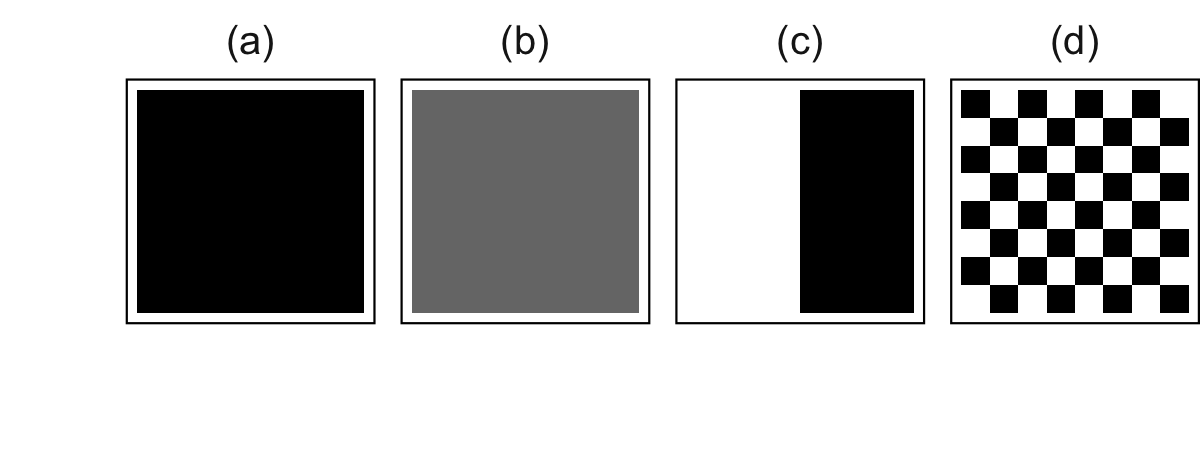
\includegraphics[width=.7\linewidth]{figs/checkerboard.png}
		\centering
		  \begin{tabular}{c | c c c}
			  City & $H(Y)$ & $I(X,Y)$ & $J(X,Y)$ \\
			  \hline			
			  (a) & 0.0 & 0.0 & 0.0\\
			  (b) & 0.7 & 0.0 & 0.0\\
			  (c) & 0.7 & 0.7 & 0.6\\
			  (d) & 0.7 & 0.7 & 2.7\\
			  \hline  
			\end{tabular}
		\caption{Information theory and the checkboard problem: model cities with various kinds of spatial diversity can be distinguished through progressively more subtle spatial information measures.}
		\label{fig:toy}
		\end{figure}

\subsection{Measuring Socio-Spatial Complexity}

	We will now derive a measure that solves the ``checkerboard problem'' by distinguishing the toy cities (c) and (d). To motivate our methods, we  consider an idealized scenario in which we have a differentiable field $p(y|x)$ of observed probability distributions for each $x \in M \subset \R^n$, where the metric space $M$ is interpretable as the ``map'' on which we work. 

	Fix a point $x_0 \in M$ and a radius $r > 0$. Let $B_r(x_0)$ denote the ball of radius $r$ about $x_0$. Then, define the \emph{local mutual information in radius $r$} as the mutual information between $X$ and $Y$, restricted to the small ball $B_r(x_0)$ about $x_0$:
	\begin{equation}
		I_r(x_0) \triangleq \E_X[D[p(\cdot|X)\| p(\cdot|X \in B_r(x_0))]|X \in B_r(x_0)] \label{eq:local}
	\end{equation}
	Intuitively, $I_r(x_0)$ measures how much knowing the ``location'' $x$ adds to our information about the category $Y$, or, equivalently, how much the probability field $p(y|x)$ varies with $x$ in a small neighborhood of $x_0$. It is therefore a natural measure of local complexity, aligned in approach with the global mutual information but designed to detect local variation. As expected, $I_r(x_0) = 0$ if and only if $p(y|x)$ is constant for each $y$ in the ball $B_r(x_0)$; that is, if within $B_r(x_0)$ the field $p(y|x)$ resembles toy city (b) in Figure \ref{fig:toy}. In the definition \eqref{eq:local}, $r$ may be thought of as the spatial resolution at which we conduct analysis, and $I_r(x_0)$ is highly dependent on $r$. However, it is possible to show that $I_r(x_0)$ is related to a fundamental statistical property of the probability field $p(y|x)$ that is resolution-independent. Under the stated conditions, the following approximation holds: 

	\begin{equation}
		\frac{I_r(x)}{r^2} \cong \frac{1}{4} \text{trace } J_Y(x)\;, \label{eq:approx}
	\end{equation}
	where $J_Y(x)$ is the Fisher information matrix in $Y$ about $x$, defined as 
	\begin{equation}
		J_Y(x) \triangleq \E_Y\left[ (\nabla_x \log p(Y|x))(\nabla_x \log p(Y|x))^T \right]\;.
	\end{equation}
	A formal statement and proof of \eqref{eq:approx} are provided in Appendix 2. The Fisher information $J_Y$ is a fundamental quantity in statistics and information theory. From a geometric perspective, $J_Y$ provides the natural intrinsic metric in the geometric space of probability distributions parameterized by the spatial variable $x$. Equation \eqref{eq:approx} therefore expresses a relationship between the local mutual information $I_r(x)$ and the information geometry of the underlying probability field. Corresponding to the fact that $I_r(x_0)$ vanishes if and only if $p(y|x)$ is constant in $B_r(x_0)$, $J_Y(x_0) = 0$ if and only if $\nabla_x p(y|x_0) = 0$ for all $y$. This implies that $x_0$ is a stationary point, about which the probability field $p(y|x_0)$ exhibits only small (2nd order or smaller) changes with respect to changes in $x$. 

	Since the Fisher information is a strictly local measure of statistical variability around $x$, we can aggregate the Fisher information to derive a measure of average local variability. The \emph{mean local information} is 
	\begin{equation}
	J(X,Y) \triangleq \E_X[\text{trace }J_Y(X)] \label{eq:def_J}
	\end{equation} 
	As demonstrated in Figure \ref{fig:toy}, $J(X,Y)$ distinguishes cities (c) and (d), thereby addressing the ``checkerboard problem'' head on. We propose the aggregate quantity $J(X,Y)$ as a third  measure--alongside the entropy $H(Y)$ and mutual information $I(X,Y)$-- as a tool for the information-theoretic structure of spatial compositional complexity. 

	We note that, since 
	\begin{align}
		\text{trace } J_Y(x) &=  \sum_i \E_Y\left[ \left(\frac{1}{p(Y|x)} \frac{\partial p(Y|x)}{\partial x_i}\right)\right]^2\;
	\end{align}
	may be viewed as a weighted norm of the gradient $\nabla_x p(Y|x)$, the quantity 
	\begin{align}
		J(X,Y) &= \E_X[\text{trace } J_Y(X)] \\
		&= \int_M \text{trace } J_Y(X) d\prob_X
	\end{align}
	may be viewed as a cousin to total variation measures often encountered in analysis. 

	The application of this methodology to a discrete data set is conceptually simple. For a given set of tracts, overlay an evenly spaced grid of radius $r$, and measure the mutual information $I_r(x)$ in each grid cell. Then, when data and grid resolutions are sufficiently high, $4I_r(x) / r^2$ approximates the quantity $\text{trace }J_Y(x)$, which can then be aggregated across the data set. We provide a more formal statement of this computation in the appendix. 

\subsection{Information Measures and Segregation Studies}

	Considerable attention has been paid to relating segregation indices to intuitive concepts of diversity and segregation. We note here that the mutual information $I(X,Y)$ and mean local information $J(X,Y)$ correspond closely to the two dimensions of segregation formulated in \cite{Reardon2002}. The authors of \cite{Reardon2002} describe \emph{evenness} as ``the extent to which groups are similarly distributed in residential space'' (page 126), and \emph{exposure} as ``the extent that members of one group encounter members of another group...in their local spatial environments.'' The mutual information $I(X,Y)$ may be viewed as a measure of (lack of) evenness, since to say that groups are similarly distributed in residential space is to say that knowing a spatial location conveys little about the race of the people who live there. Large $I(X,Y)$ reflects highly uneven distributions of demographic groups. Complementarily, the mean local information $J(X,Y)$may be viewed as a measure of spatial exposure \emph{for a fixed level of} $I(X,Y)$, as is illustrated by cities (c) and (d) in \ref{fig:toy}. Though distinct, these dimensions are not independent. To see this, note that the most thorough kind of exposure is achieved when $I(X,Y) = J(X,Y) = 0$, as in city (b). Since the concept of exposure only applies in a city with spatial differences, $J(X,Y)$ must be considered jointly with $I(X,Y)$ as a measure of spatial exposure. 

	There has also been much work showing the desirable properties of various segregation indicies. To give a brief sampling, indices should be invariant to changes in overall population size; they should decrease when populations ``even themselves out,'' and they should behave predictably under aggregation. Since we are presenting $I(X,Y)$ and $J(X,Y)$ as a suite of complementary information measures, we consider each in turn. The author of \cite{Roberto2015a} shows that the mutual information $I(X,Y)$ (which she calls the ``Divergence Index'') satisfies these and other desirable properties, generally as well or better than existing alternatives. We highlight one property of $I(X,Y)$ for special note, as this property will be central to our development of natural neighborhood identification. The principle of ``additive decomposability'' \cite{Reardon2002} stipulates that, when the data is grouped along either racial or spatial axes, a good segregation index should split into ``within group'' and ``between group'' components. In the context of the mutual information $I(X,Y)$, additive decomposability is simply the familiar chain rule of mutual information. For concreteness, let $C$ be a random variable giving the cluster label of location $X$; importantly, $C$ is completely determined by $X$. Then, the chain rule expresses additive decomposability as 
	\begin{equation}
		I(X,Y) = I(C,Y) + I(X,Y|C)\;; \label{eq:information_decomp}
	\end{equation}
	i.e. the information I have about $Y$ given that I know $X$ is equal to the information I have if I first learn the cluster $C$, plus the amount of additional information I gain if I subsequently learn the exact location $X$ as well. The first term is interpretable as the between-group information, while the second is interpretable as the within-group information. It is therefore comparable to various ``sum of squares'' decompositions that frequently appear in classical statistics. Indeed, it is possible to show that, when the differences between locations are small, the mutual information can be interpreted as a variance, in which case \eqref{eq:information_decomp} expresses the sum of squares composition directly. A similar version of the chain rule expresses additive decomposability for aggregation of racial groups rather than spatial locations. 

	What of $J(X,Y)$? Below, we provide a brief overview of the properties of $J(X,Y)$. $J(X,Y)$ possesses a variety of intuitive properties, and those that it does not possess either underscore the importance of reading it in conjunction with $I(X,Y)$ or do not apply to explicitly spatial measures.  See \cite{Reardon2002,Reardon2004} for further discussion of these criteria. The mean local information $J(X,Y)$ satisfies: 
	\begin{description}
		\item[Organizational Equivalence:] Both the theoretical definition \eqref{eq:def_J} or the procedure to compute it from tract data remain unchanged when a tract is subdivided into smaller tracts, each of which with identical demographic structure. 
		\item[Size and Density Invariance:] Since $J(X,Y)$ is completely determined by the marginal distribution $p(X,Y)$, it is invariant under changes in population density. 
		\item[Additive Group Decomposability:] When demographic groups are aggregated into super-groups, the chain rule of mutual information applied to the demographic variable $Y$ provides an an additive decomposition of the form $J(X,Y) = J(X,G) + J(X,Y|G)$, which can be interpreted as the sum of a between-groups term and a within-groups term as needed.   
		\item[Scale Interpretability:] We have $J(X,Y) = 0$ if and only if $p(Y|X)$ is constant on each connect component of the metric space $M$. When only one connected component exists, this implies that every locale has the same demographic structure as the global environment. When multiple connected components exist (e.g. the city is divided by a river), demographics must be constant in space on each side of the division. $J(X,Y)$ does not satisfy the additional condition of achieving its maximum value when all locales are monoracial, but this point only emphasizes that $J(X,Y)$ and $I(X,Y)$ should be read jointly. When all locales are monoracial, $I(X,Y)$ achieves its maximum value and $J(X,Y) = 0$. 
		\item[Boundary Independent:] $J(X,Y)$ is defined in terms of a continuous underlying probability distribution $p(X,Y)$, rather than arbitrarily-defined tracts. In computational practice, $J(X,Y)$ is indeed sensitive to the boundaries supplied with the data; however, \eqref{eq:approx} guarantees that this sensitivity vanishes as the resolution grows sufficiently small.  
		\item[Exchanges:] Exchanges that tend to ``smooth out'' demographic distributions in space reduce both $I(X,Y)$ and $J(X,Y)$.  
	\end{description}
	The mean local information $J(X,Y)$ fails to one of the criteria enumerated in \cite{Reardon2002,Reardon2004}; that of \textbf{additive spatial decomposability}. This criterion states that ``If X spatial subareas are aggregated into Y larger spatial areas, then a segregation measure should be decomposable into a sum of within- and between-area components'' \cite{Reardon2004}, page 136. However, considering that we have imposed additional spatial structure on our model, this criterion does not appear to be motivated. Consider, for example, Figure \ref{fig:decomposability}. Aggregating the two central regions transforms (e) into (f), erasing all spatial variability. Any measure should therefore have a between-groups component equal to 0. On the other hand, the within-groups component can only consider the middle white/black boundary between the central two regions. The sum of the between-groups and within-groups components must therefore consist only in information included in the middle boundary. However, the spatial variability in city (e) is not exhausted by this middle boundary; there are a total of six other frontiers of racial difference that should be considered in any spatial segregation measure. We therefore content that additive decomposability is a desideratum of nonspatial measures (it is satisfied by $I(X,Y)$), but not of explicitly spatial ones. 
	\begin{figure}
		\centering
		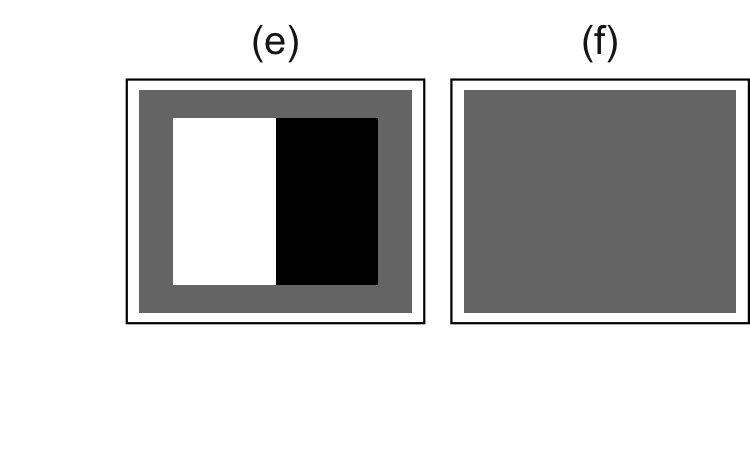
\includegraphics[width=.5\textwidth]{figs/decomposability.png}
		\caption{A problem with additive spatial decomposability: aggregating the inner two regions transforms (e) into (f), smoothing out all spatial variability. A ``between groups'' term must therefore vanish, while a ``within-groups'' term considers only the inner boundary; not the outer ones.}
		\label{fig:decomposability}
	\end{figure}
	We have not exhausted the full complement of desiderata for segregation measures. However, many of the remaining ones -- such as composition invariance -- are either vague or controversial, and we will not consider further. 

\subsection{Identifying Natural Neighborhoods}
	
	Equation \eqref{eq:information_decomp} motivates a simple scheme for identifying natural neighborhoods based on maximizing the between-group term $I(C,Y)$. If all I had access to were the cluster labels $C$ and not the locations $X$, then the information I had about $Y$would be $I(C,Y)$. A ``good'' clustering therefore maximizes the between-cluster information $I(Y,C)$, which entails minimizing the within-cluster information $I(X,Y|C)$. Solving this problem exactly is a challenging discrete optimization problem, and may not be computationally tractable. We can, however, construct a greedy algorithm which leads to satisfactory results. Suppose that we face the problem of choosing a pair of tracts $\{i*,j*\}$ to cluster together. The reduction in information associated with aggregating the locations $I$ into a single cluster is 
	\begin{align}
		d(i,j) &\triangleq  \sum_{k \in \{i,j\}} p(X = k)D[p(Y|X = k)\| p(Y|X \in \{i,j\})] \\
		&- p(X\in \{i,j\})D[p(Y|X\in \{i,j\}) \| p(Y)] \label{eq:info_dist}
	\end{align}
	where $p(Y) = \sum_{x} p(x,Y)$ is the global marginal distribution. the first term is the information associated with the two separate tracts, while the second is the information associated with a merged tract. Equation \eqref{eq:info_dist} defines a natural information distance between locations $i$ and $j$. Like the KL divergence, this distance is strictly nonnegative; unlike the KL divergence, it is symmetric, and defines an axiomatic metric on the space of tracts. Importantly, we can therefore use the distance $d(i,j)$ as a dissimilarity measure for the purposes of clustering. Our greedy procedure is simple: at each iteration, determine
	\begin{equation}
		(i^*,j^*) = \argmin_{i \text{neighbors} j} d(i,j),
	\end{equation}
	and then combine $i^*$ amd $j^*$ into a single tract, repeating until only one cluster remains. This procedure defines a form of agglomerative hierarchical clustering distinguished by two characteristics: its spatial constraints and its pursuit of minimal information loss at each step. As a greedy algorith, it possesses no guarantees for optimal solutions, but in practice its performance leads to intuitive, racially-coherent regions. It thereby enables a study of spatial difference using non-arbitrarily-defined regions. 







\section{Findings}
	\nocite{Bivand2014b,Bivand2014a,Bivand2014} % need to cite the census in here too

\subsection*{Data Used}
	We assembled block-group level data from the 2010-2014 American Community Survey (ACS), conducted by the U.S. Census Bureau, on race and ethnicity for counties housing 51 large US cities. We then aggregated the detailed racial and ethnic groups into five meta-categories: `Asian', `Black', `Hispanic', `Other', and `White'.

\subsection*{Information Measures}

	 For each city, we computed the entropy $H(Y)$ and the mutual information $I(X,Y)$. To compute the estimated aggregate Fisher information $J(X,Y)$, we tiled the map with a hexagonal grid of cell radius 0.5km. We then computed the estimated mutual information within each grid cell, and averaged the results weighted by population population. A technical specification of this approach is provided in Appendix 1, and an illustration of it in Figure \ref{fig:method}. 

	 \begin{figure}
		\centering
		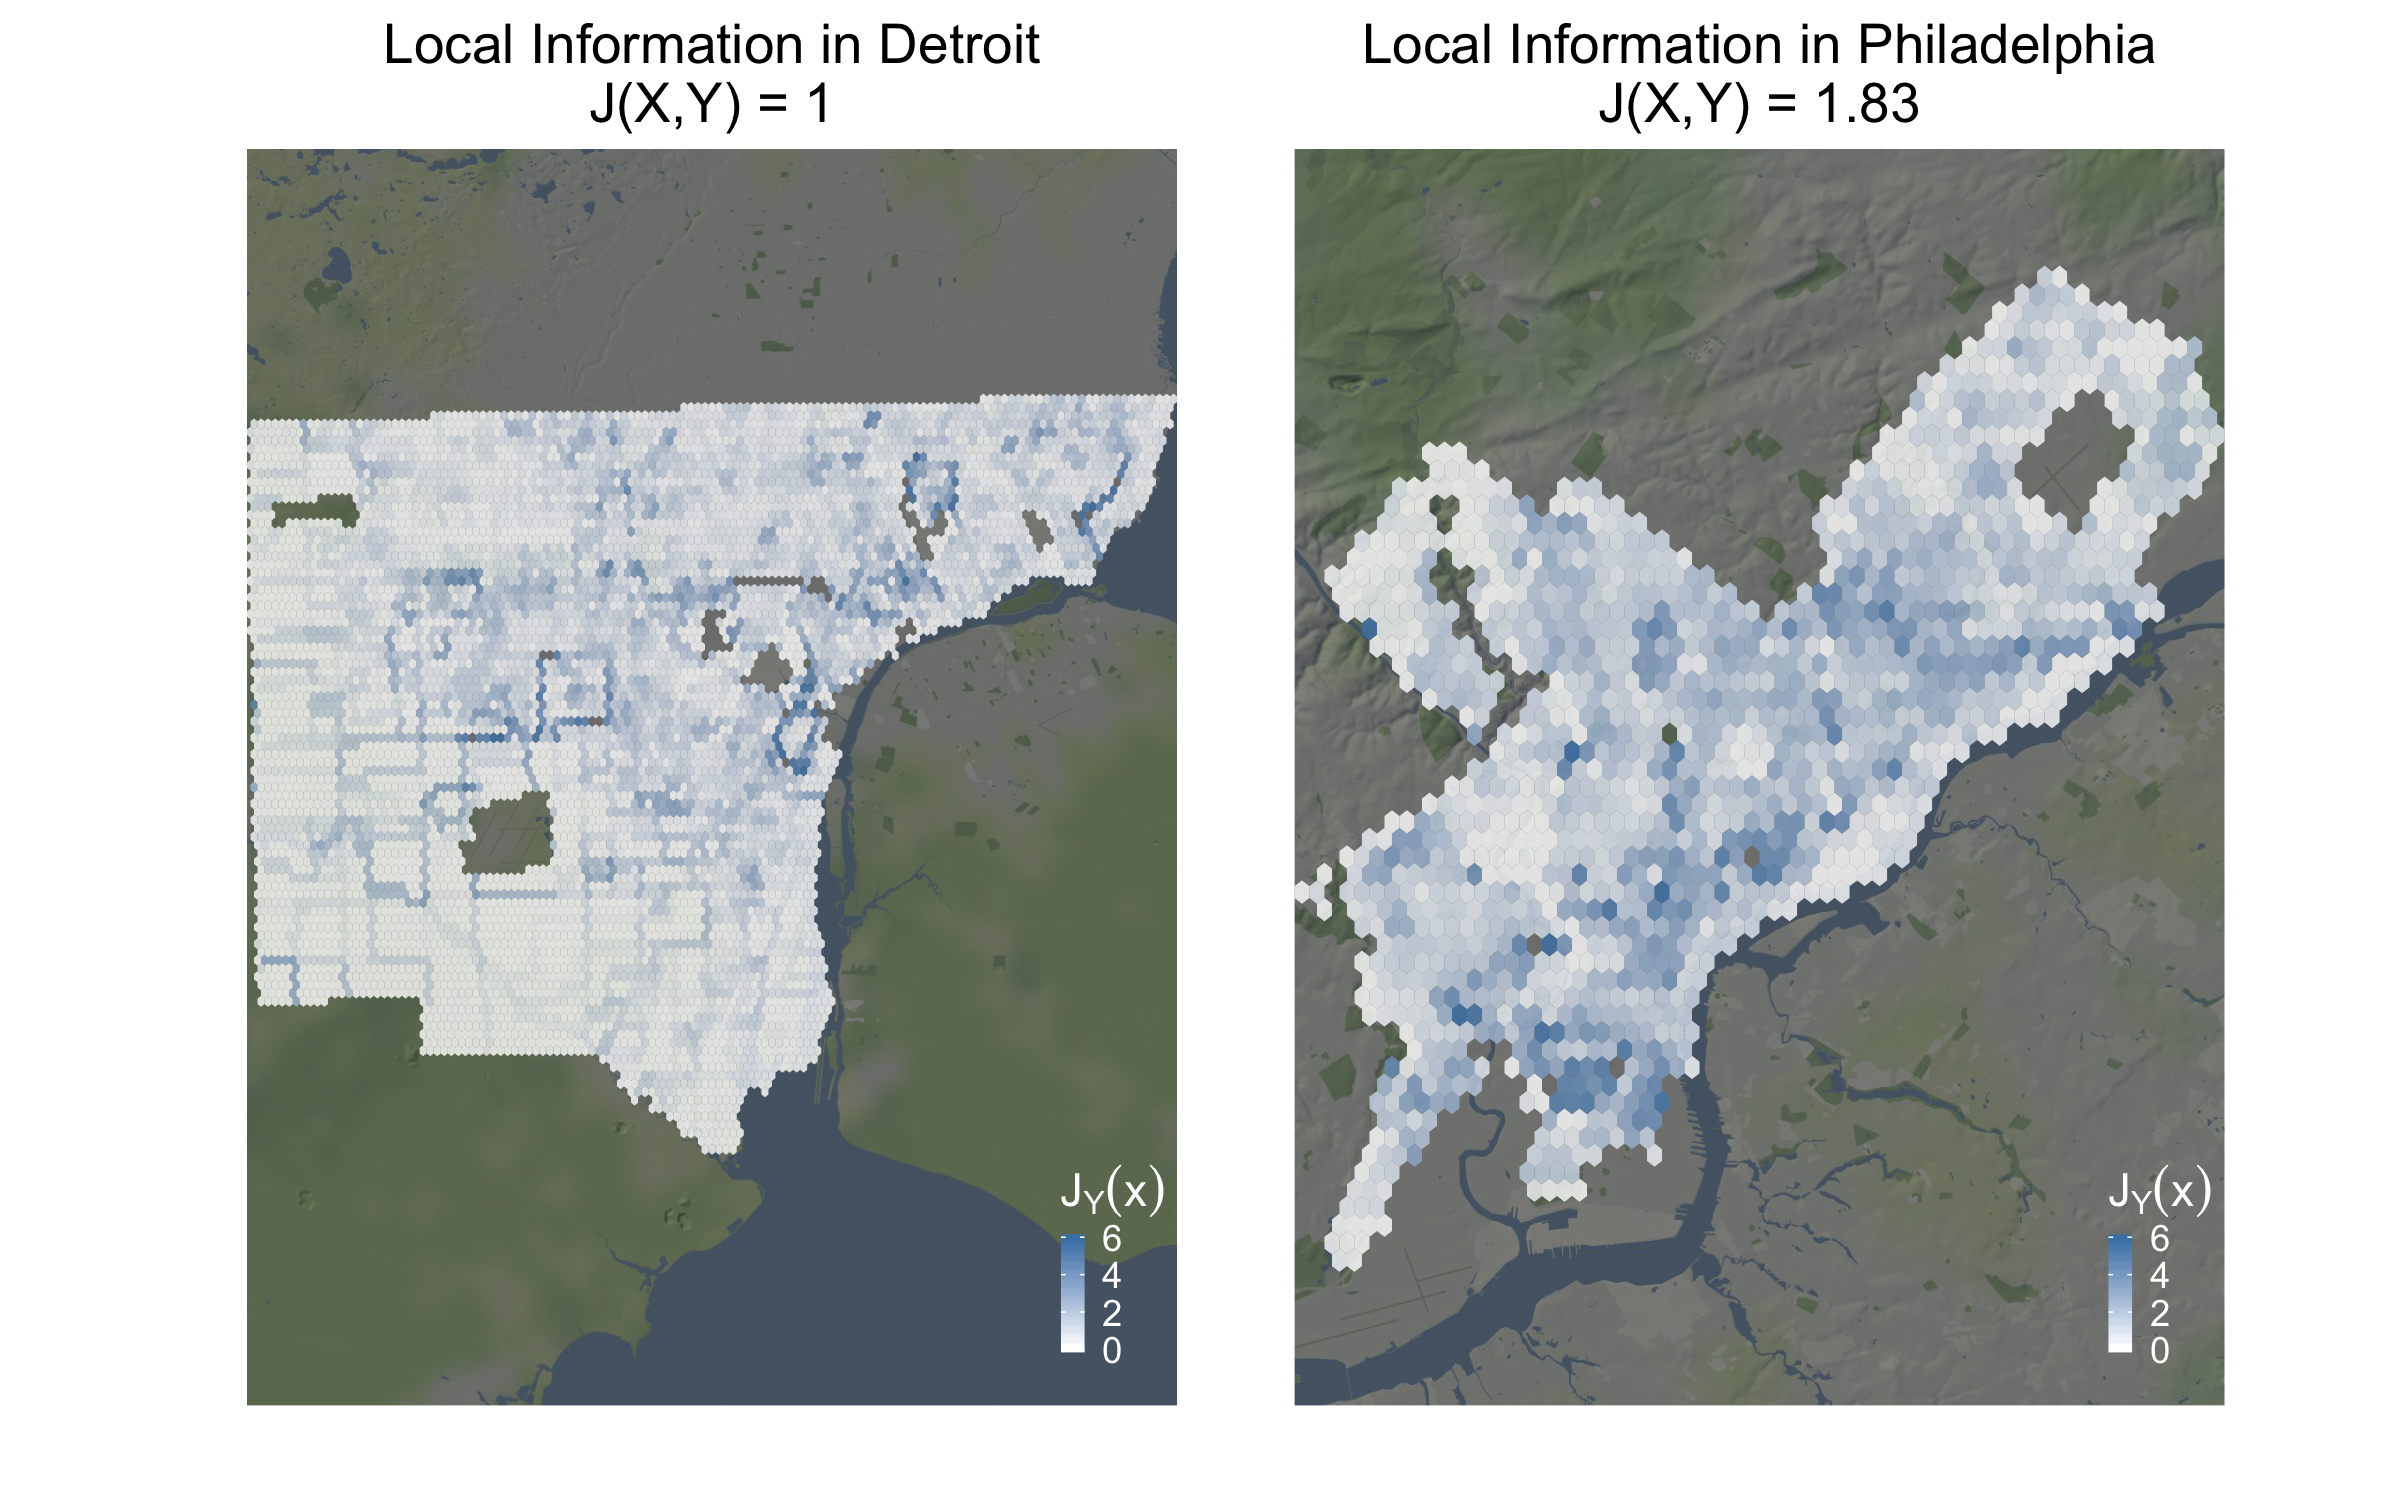
\includegraphics[width=.8\textwidth]{figs/method_illustration.png}
		\caption{Illustration of methodology for estimating local information in Suffolk County, MA (Boston). We first cover the map in a hexgrid, and compute the mutual information within each hex from the Census tracts that overlap the hex, weighted by density. }
		\label{fig:method}
	\end{figure}


	Figure \ref{fig:info_cross} shows the relationship of the mutual information (or evenness) $I(X,Y)$ and mean local information (or exposure) $J(X,Y)$. The global positive trend reflects the fact that global spatial variability is a prerequisite for local variability: if the city is uniform (like Figure \ref{fig:toy}(a)), then no local differences either exist.  On the other hand, there are substantial variations in $J(X,Y)$ even in cities with comparable global variability $I(X,Y)$. For example, the cities of Detroit and Philadelphia provide a striking contrast. While they have mutual information $I(X,Y)$, Philadelphia's mean local information $J(X,Y)$ is substantially higher. This reflects the fact that Detroit is composed of large, highly-segregated, monoracial neighborhoods, whereas Philadelphia has a much more fine-grained, intricate neighborhood structure. These patterns illustrate how combinations of the information measures $H(Y)$, $I(X,Y)$, and $J(X,Y)$ can be used to construct taxonomies diversity for American cities. It may be useful summarise the two measures by calling cities close to the bottom-right ``most segregated'', but we recommend reporting both $I(X,Y)$ and $J(X,Y)$. It is best to compare $J(X,Y)$ only between cities with similar $I(X,Y)$; thus, while it may be right to say that Detroit has lower levels of exposure than Phildelphia, when comparing Detroit to Baltimore it should be kept in mind that Baltimore is more even in its overall sociospatial structure. 
	\begin{figure}
		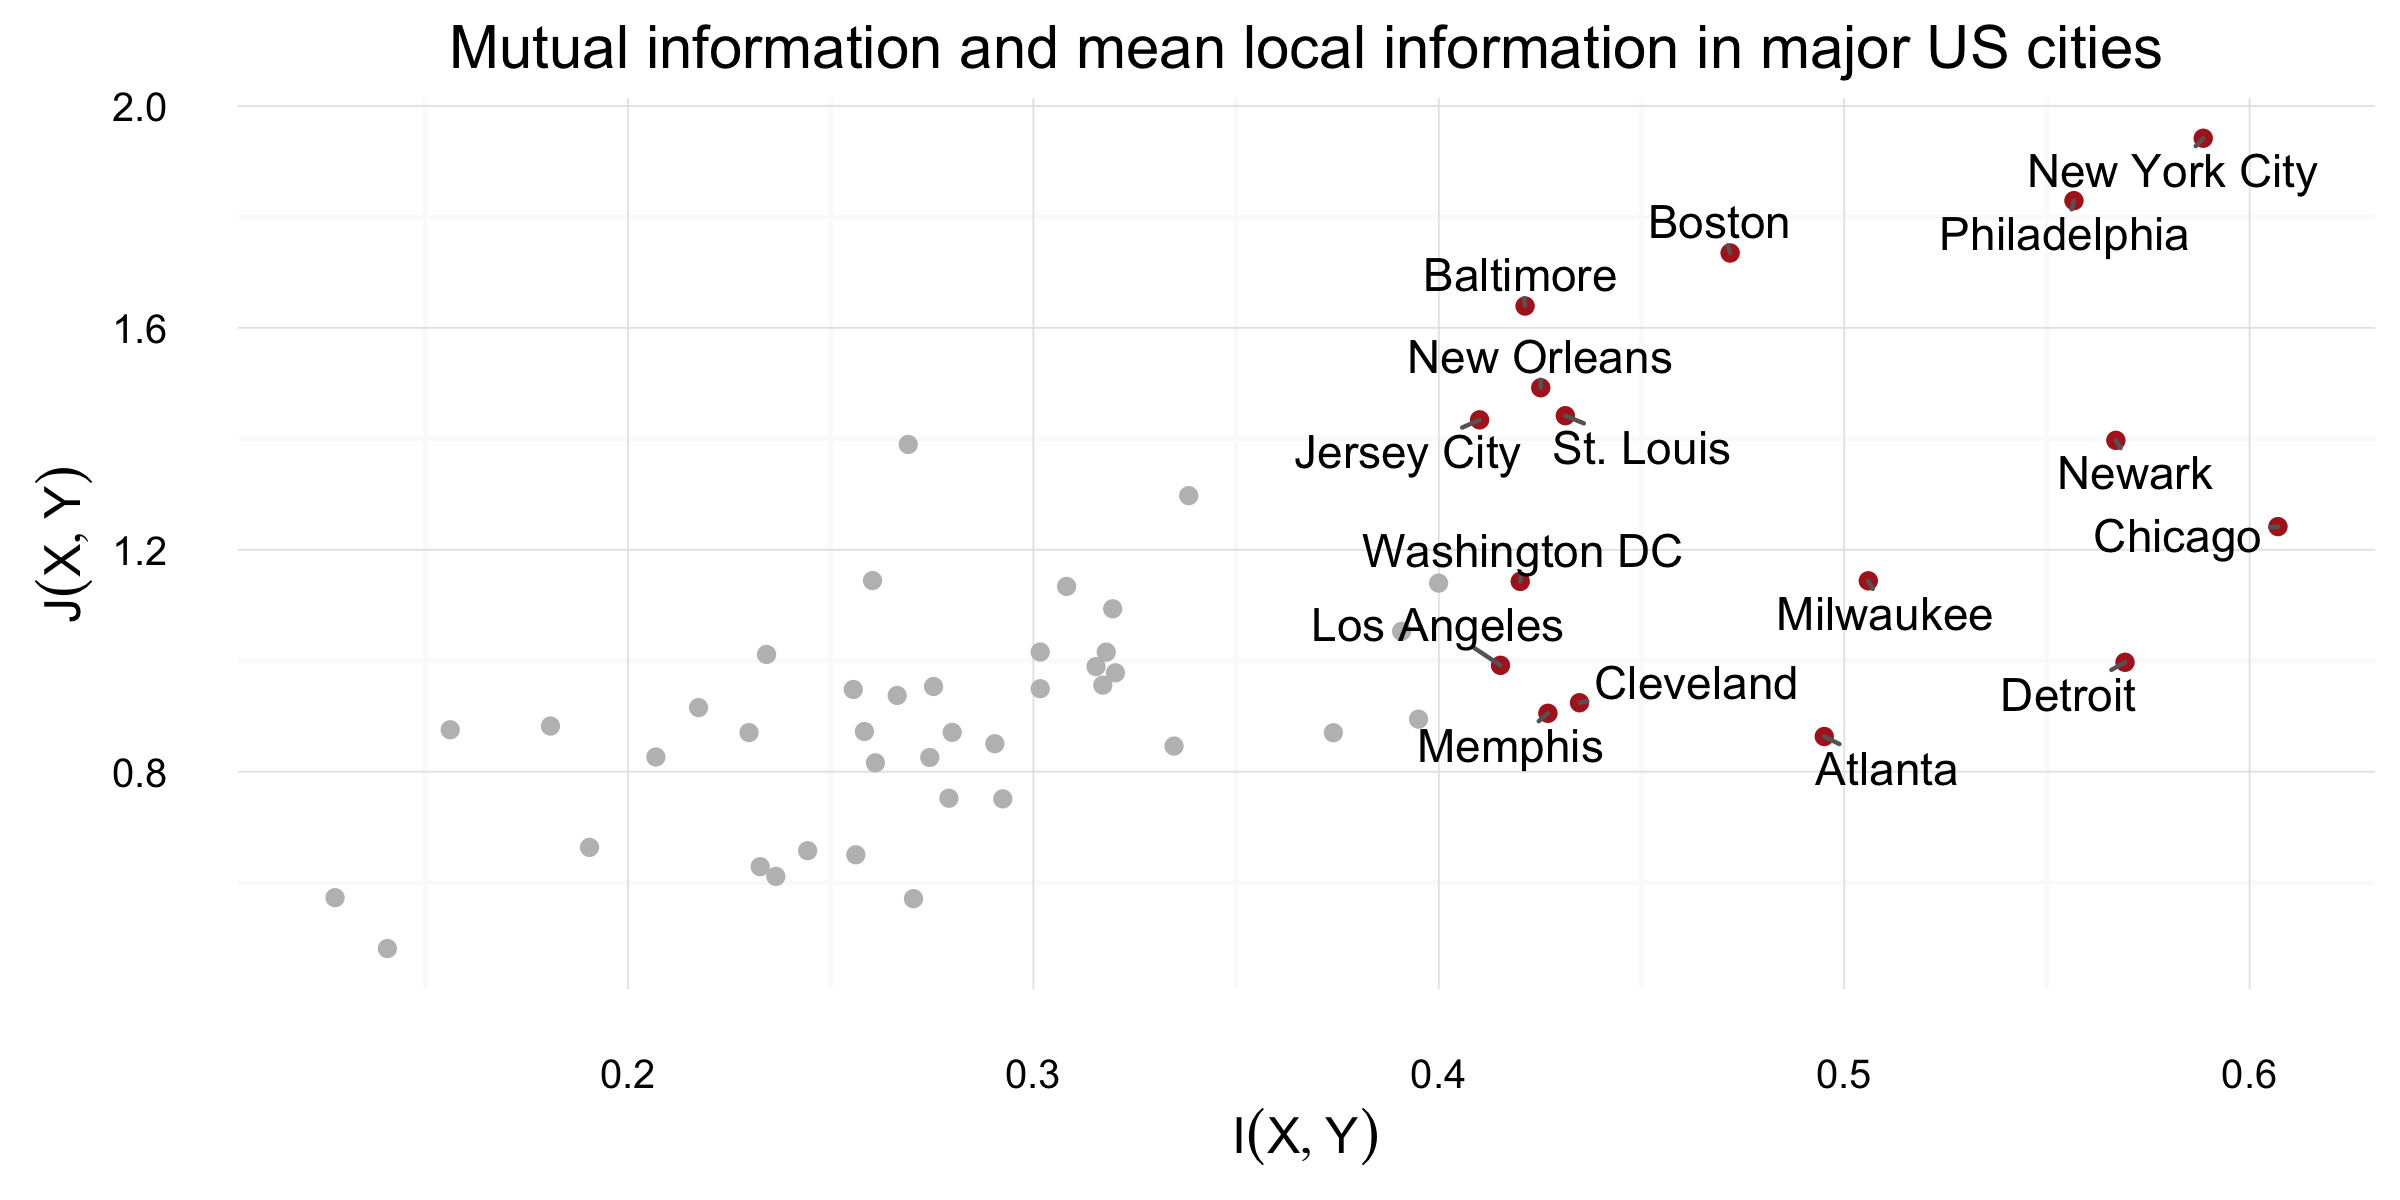
\includegraphics[width=1\textwidth]{figs/mutual_fisher.png}
		\caption{Relationship of global mutual information $I(X,Y)$ and mean local information $J(X,Y)$.} 
		\label{fig:info_cross}
	\end{figure}	


	
	\begin{figure}
		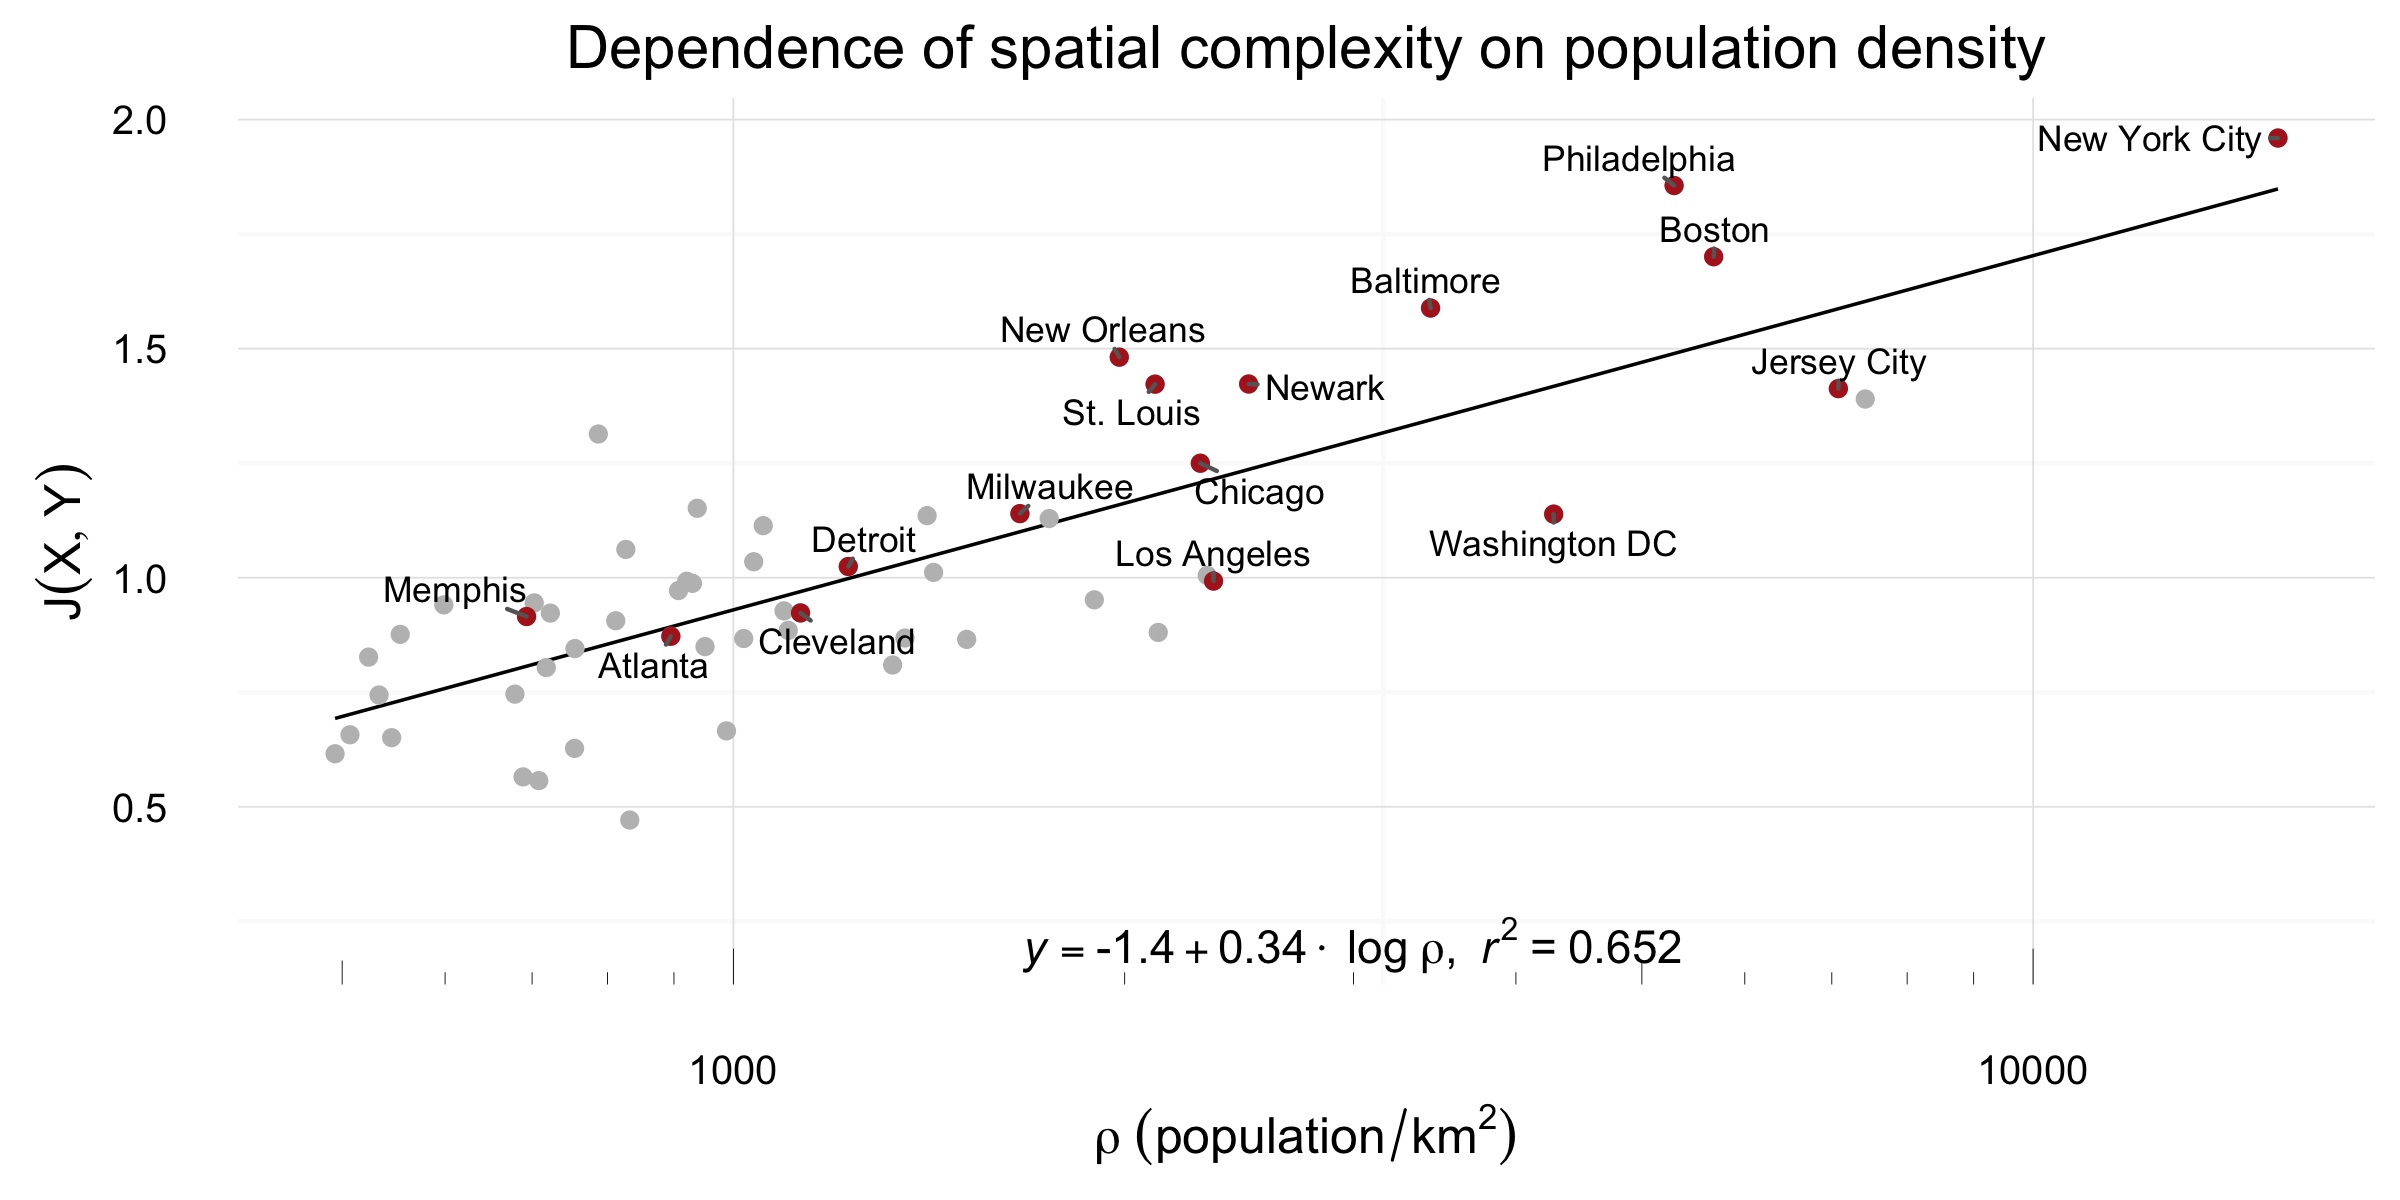
\includegraphics[width=1\textwidth]{figs/density_fisher.png}
		\caption{The mean local information $J(X,Y)$ scales with the logarithm of population density.}
		\label{fig:density}
	\end{figure}	

	Intriguingly, the mean local variability $J(X,Y)$ appears obey a scaling relation with respect to urban density. In Figure \ref{fig:density}, we plot $J(X,Y)$ against the population density $\rho$ of our studied cities. It appears that $J(X,Y)$ grows linearly with the logarithm of density. We interpret this trend as reflecting a compression of social space in dense urban areas: the same structure of racial variability fits into much less geographical area in New York than in Phoenix. One aspect of diversity in large, dense cities is that one need walk much less distance in order to reach a neighborhood with substantially different racial trends than one's own. It may be of interest for later studies to consider why this trend might arise through dynamical processes of urban formation. 
	 
		

\subsection*{Learning From Natural Neighborhoods}

	Figure \ref{fig:cluster_map} shows an illustrative clustering of Wayne County (housing the city of Detroit) into six regions using the greedy information maximization procedure defined by equation \eqref{eq:info_dist}. The procedure cleanly divides the city into racially coherent zones. Cluster A is predominantly white and B predominantly black, demarcating the major racial divide in the city. Cluster C is a small transitional zone in which the two races overlap. Clusters D and E are the demographically distinct independent cities of Hamtramck and Grosse Pointe, respectively, while Cluster F is a Hispanic community known as Mexicantown. The existence of clusters like C reflects that not every racially coherent tract is interpretable as a ``neighborhood''; some may be more naturally thought as transitions between neighborhoods. 
	
	\begin{figure}
		\centering
		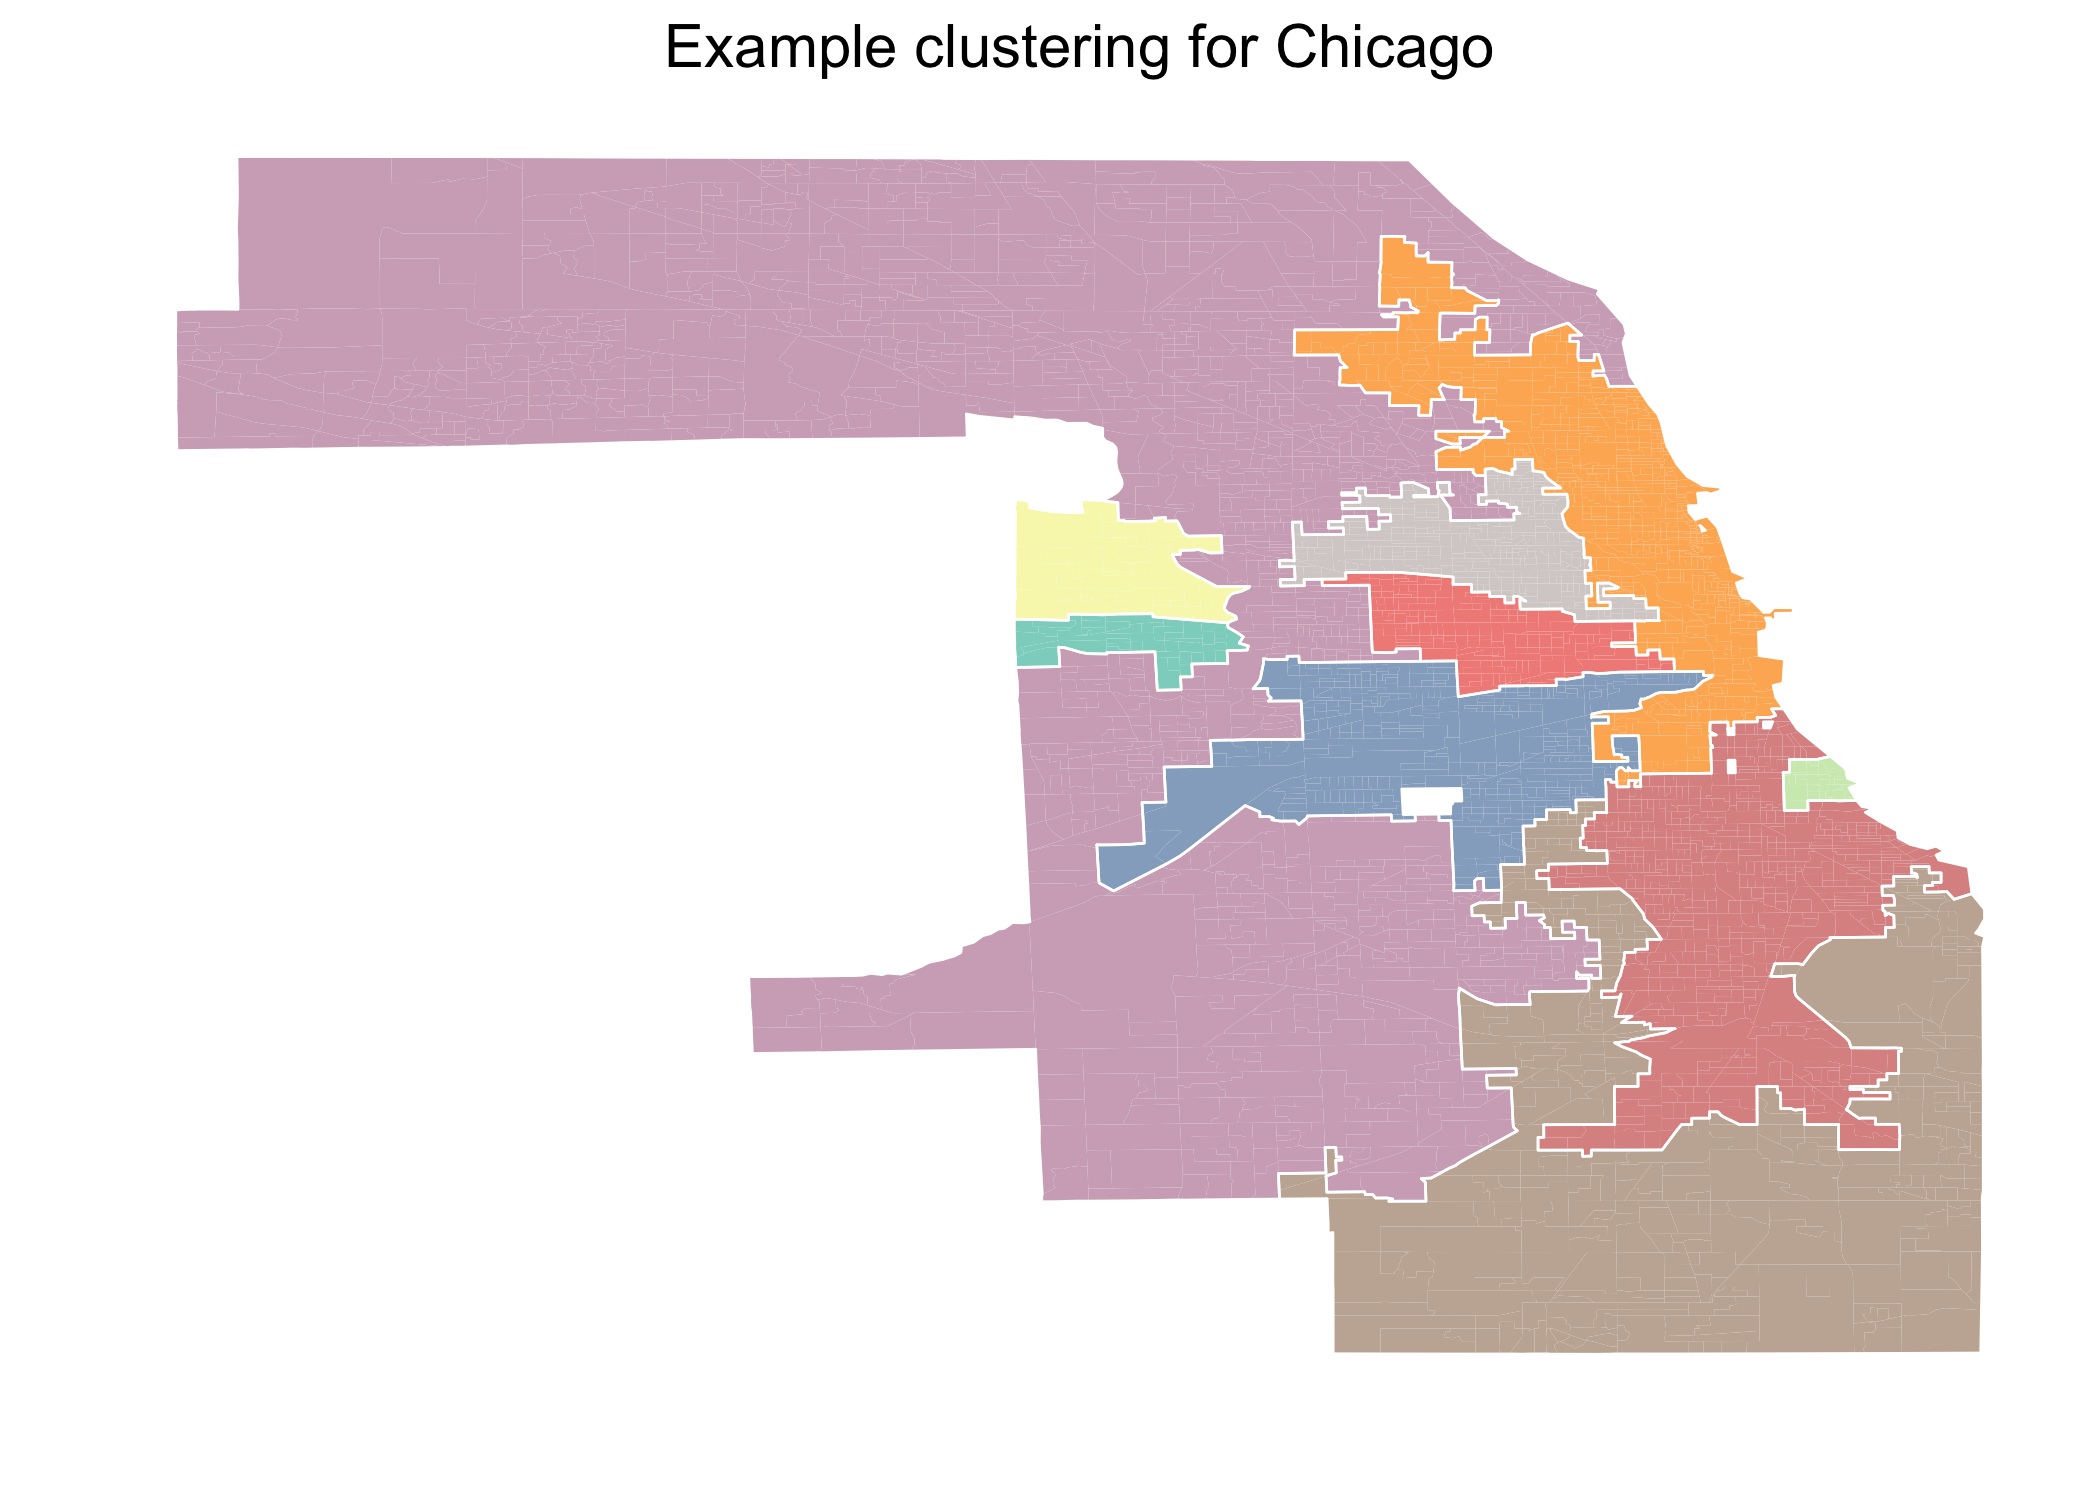
\includegraphics[width=\textwidth]{figs/example_cluster_map.png}
		\caption{Clustering of Detroit into 6 neighborhoods based on race.}
		\label{fig:cluster_map}
	\end{figure}		

	Cities vary sharply in the level of cluster detail needed to convey equal amounts of demographic information. Figure \ref{fig:clusters} shows example cluster divisions for four major cities. Each clustering conveys approximately equal demographic information, as measured by the mutual information $I(C,Y)$ between cluster labels and racial distribution. In sharply segregated Atlanta, just two clusters--one predominantly white, the other predominantly black--suffice to convey as much information as five in Boston, where the clusters are substantially more nuanced. Boston's Cluster A is predominantly white, cluster D majority Hispanic, and cluster E majority black. Cluster B is again majority white, but is distinct in that its minority citizens are almost all Hispanic. Cluster C is approximately equally black, Hispanic, and white. 

	Clusterings such as those shown in Figure \ref{fig:clusters} shed useful light on traditional concerns in the study of segregation. We have already argued that $I(X,Y)$ and $J(X,Y)$ naturally encode the high-level ideas of evenness and exposure endorsed by \cite{Reardon2004}. We now consider the further concepts of clustering and concentration. According to \cite{Massey1988}, ``\emph{clustering} measures the degree to which minority areas are located adjacent to one another'' and ``\emph{concentration} refers to the degree of a group's agglomeration in urban space'' (pages 309-310). When areas with similar racial composition are located close to one another, fewer spatial clusters are necessary to convey equivalent information about racial trends. Thus, \ref{fig:clusters} suggests that Atlanta is more clustered than Boston, a suggestion that we can quantify using the AUC methodology developed below. The concept of concentration invites us to consider the composition and density of each cluster. In Detroit, for example, whites make up 70\% of ``their'' Cluster A, while black residents make up a full 86\% of ``their'' Cluster B. Cluster B is also more concentrated in that it is more densely populated than Cluster A: it contains 34\% of the Detroit's population, but accounts for just 19\% of land in the analyzed area. This makes Cluster B more than twice as dense as Cluster A. Thus, in Detroit, ``black'' neighborhoods tend to be more racially homogeneous and more densely packed in urban space than ``white'' ones. Finally, we note that these clusterings allow us to examine the somewhat abstract concept of ``exposure'' in considerable detail. Figure \ref{fig:clusters} indicates that across all cities, Asians are much more likely to be found in predominantly white clusters than they are in predominantly black or Hispanic ones, indicating significant spatial integration between these two groups. In Chicago, some groups of Hispanics are exposed primarily to Hispanics and other whites (Cluster B), while other groups are exposed primarily to black residents (Cluster D).

	\begin{figure}
		\centering
		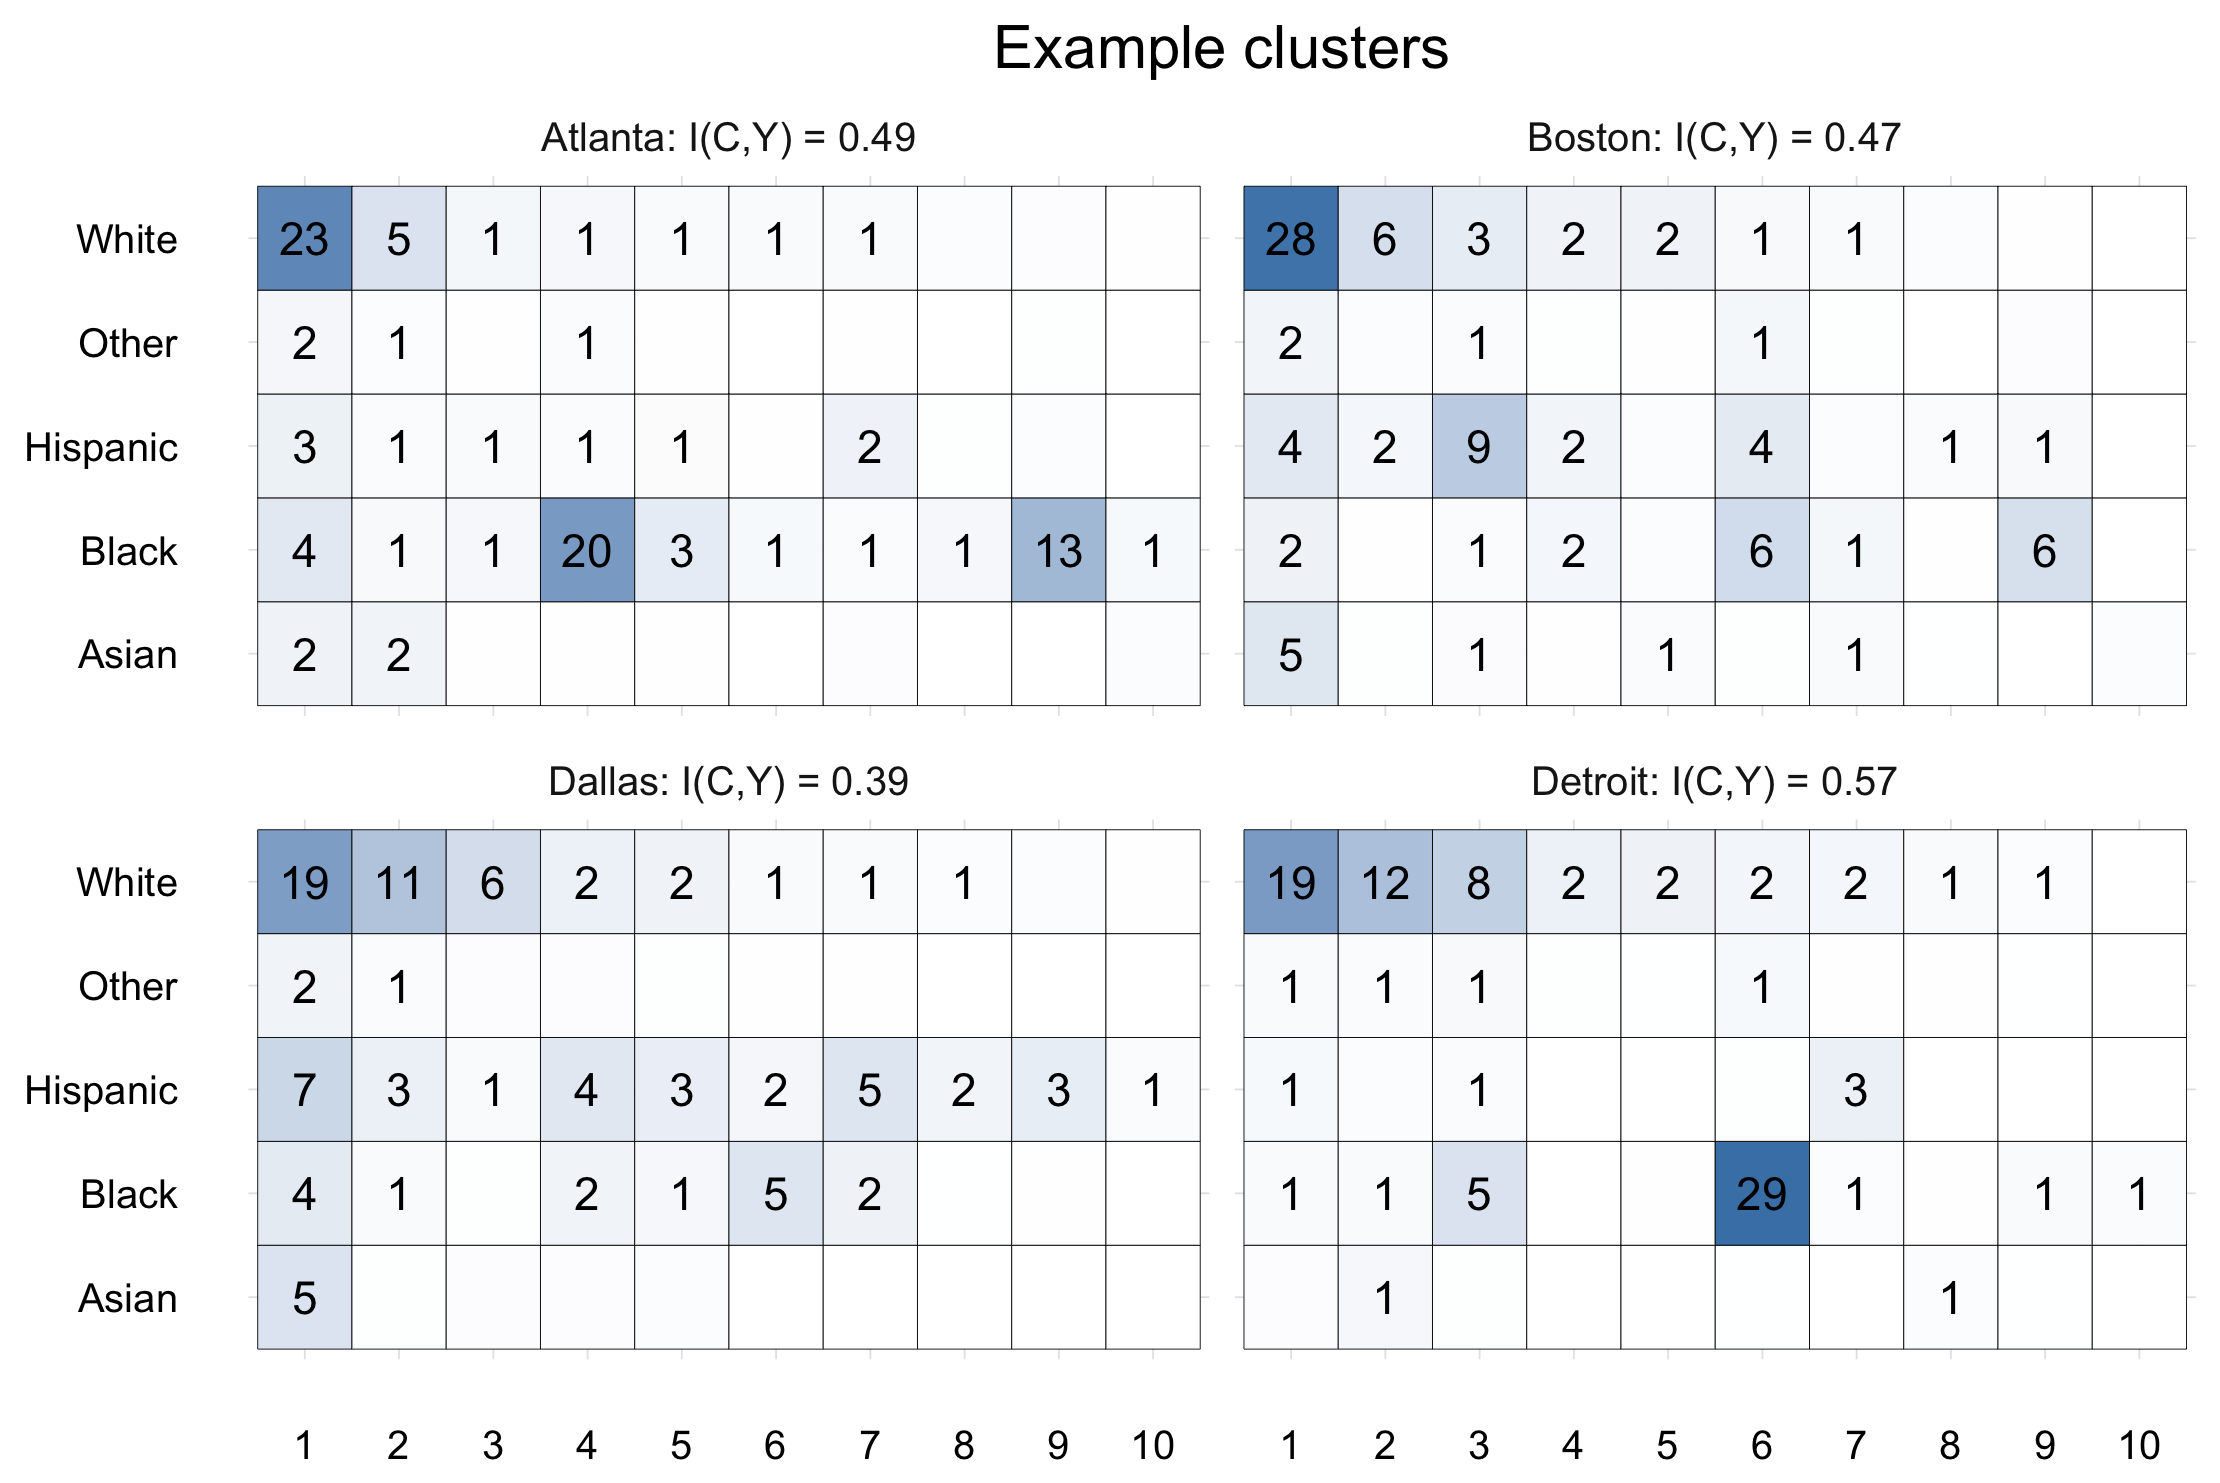
\includegraphics[width=\textwidth]{figs/example_clusters.png}
		\caption{Example clusters for different cities, and the associated mutual information contained in each. The number in each box reflects the percentage of the population in the labeled racial group and cluster. }
		\label{fig:clusters}
	\end{figure}

\subsection*{Complexity and Neighborhood Structure}

	We expect that spatially complex cities with high $J(X,Y)$ would require more complicated models in order to capture similar levels of spatiosocial structure. Testing this expectation requires a quality measure defined on cluster models for each city. The natural measure of loss for a clustering is the mutual information $I(C,Y)$ between cluster and racial labels.
		
	To develop a global evaluation of the hierarchical clustering of a city according to the method defined by \eqref{eq:info_dist}, we borrow the methodology of the ``area under the curve'' (AUC) used extensively in statistical learning. By plotting the information $I(C,Y)$ against the number of clusters $n$, we obtain a curve reflecting how the information evolves at varying scales of aggregation. Figure \ref{fig:AUC} illustrates these curves for Boston and Detroit, with $N$ plotted on a logarithmic scale.  

	\begin{figure}
		\centering
		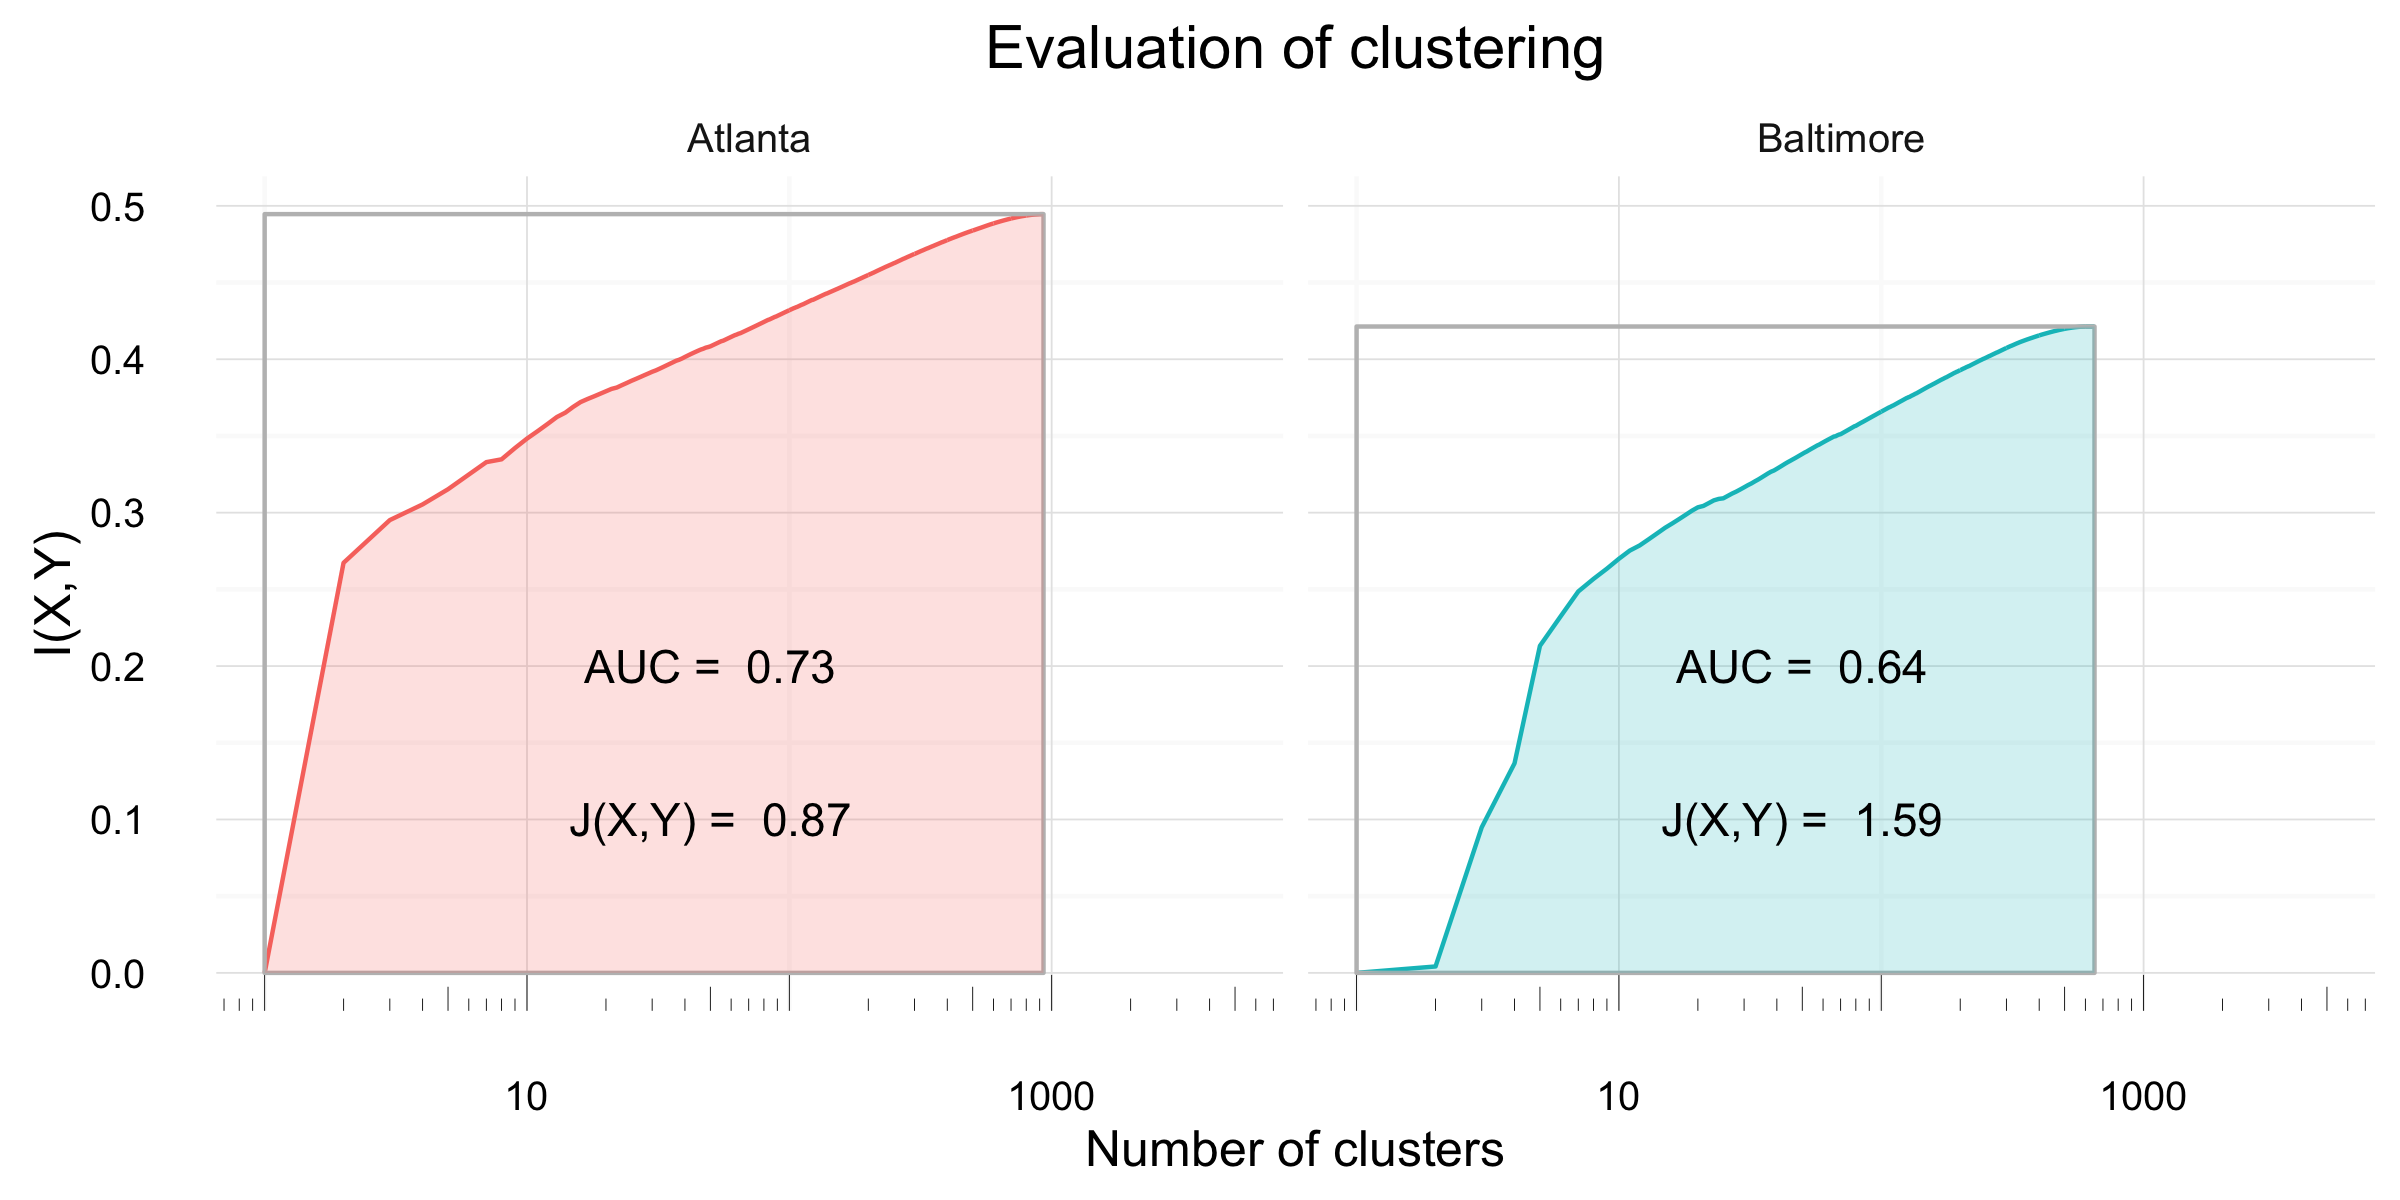
\includegraphics[width=\textwidth]{figs/AUC_illustration.png}
		\caption{Evaluation of clustering using an Area Under the Curve (AUC) metric. The AUC is the fraction of the bounding box lying under the information gain curve. Boston's AUC is smaller than Detroit's, showing that Boston's spatial complexity (measured by $J(X,Y)$) requires more complex models than Detroit's.}
		\label{fig:AUC}
	\end{figure}

	Figure \ref{fig:AUC} also shows the bounding rectangle, whose top right corner is defined by the number N of tracts in the census data set and the full mutual information $I(X,Y)$. The AUC is defined as the ratio of the shaded area in Figure \ref{fig:AUC} to the bounding rectangle. An AUC of 1 indicates that just one region carries full information; this can only occur in a city with no spatial variation, such as city (b) in \ref{fig:toy}. A larger AUC indicates that sample models with few regions capture more information about spatial variation in the city. In Detroit, there exists a clear dividing line between a predominantly white region on the west and a predominantly black region in the east. A two-cluster model therefore captures much of the information in the city, giving a high AUC of 0.74. In Boston, on the other hand, no such clear divide exists, and more complex models are necessary to capture similar amounts of information. Thus, Boston has a lower AUC of 0.67. 

	\begin{figure}
		\centering
		% 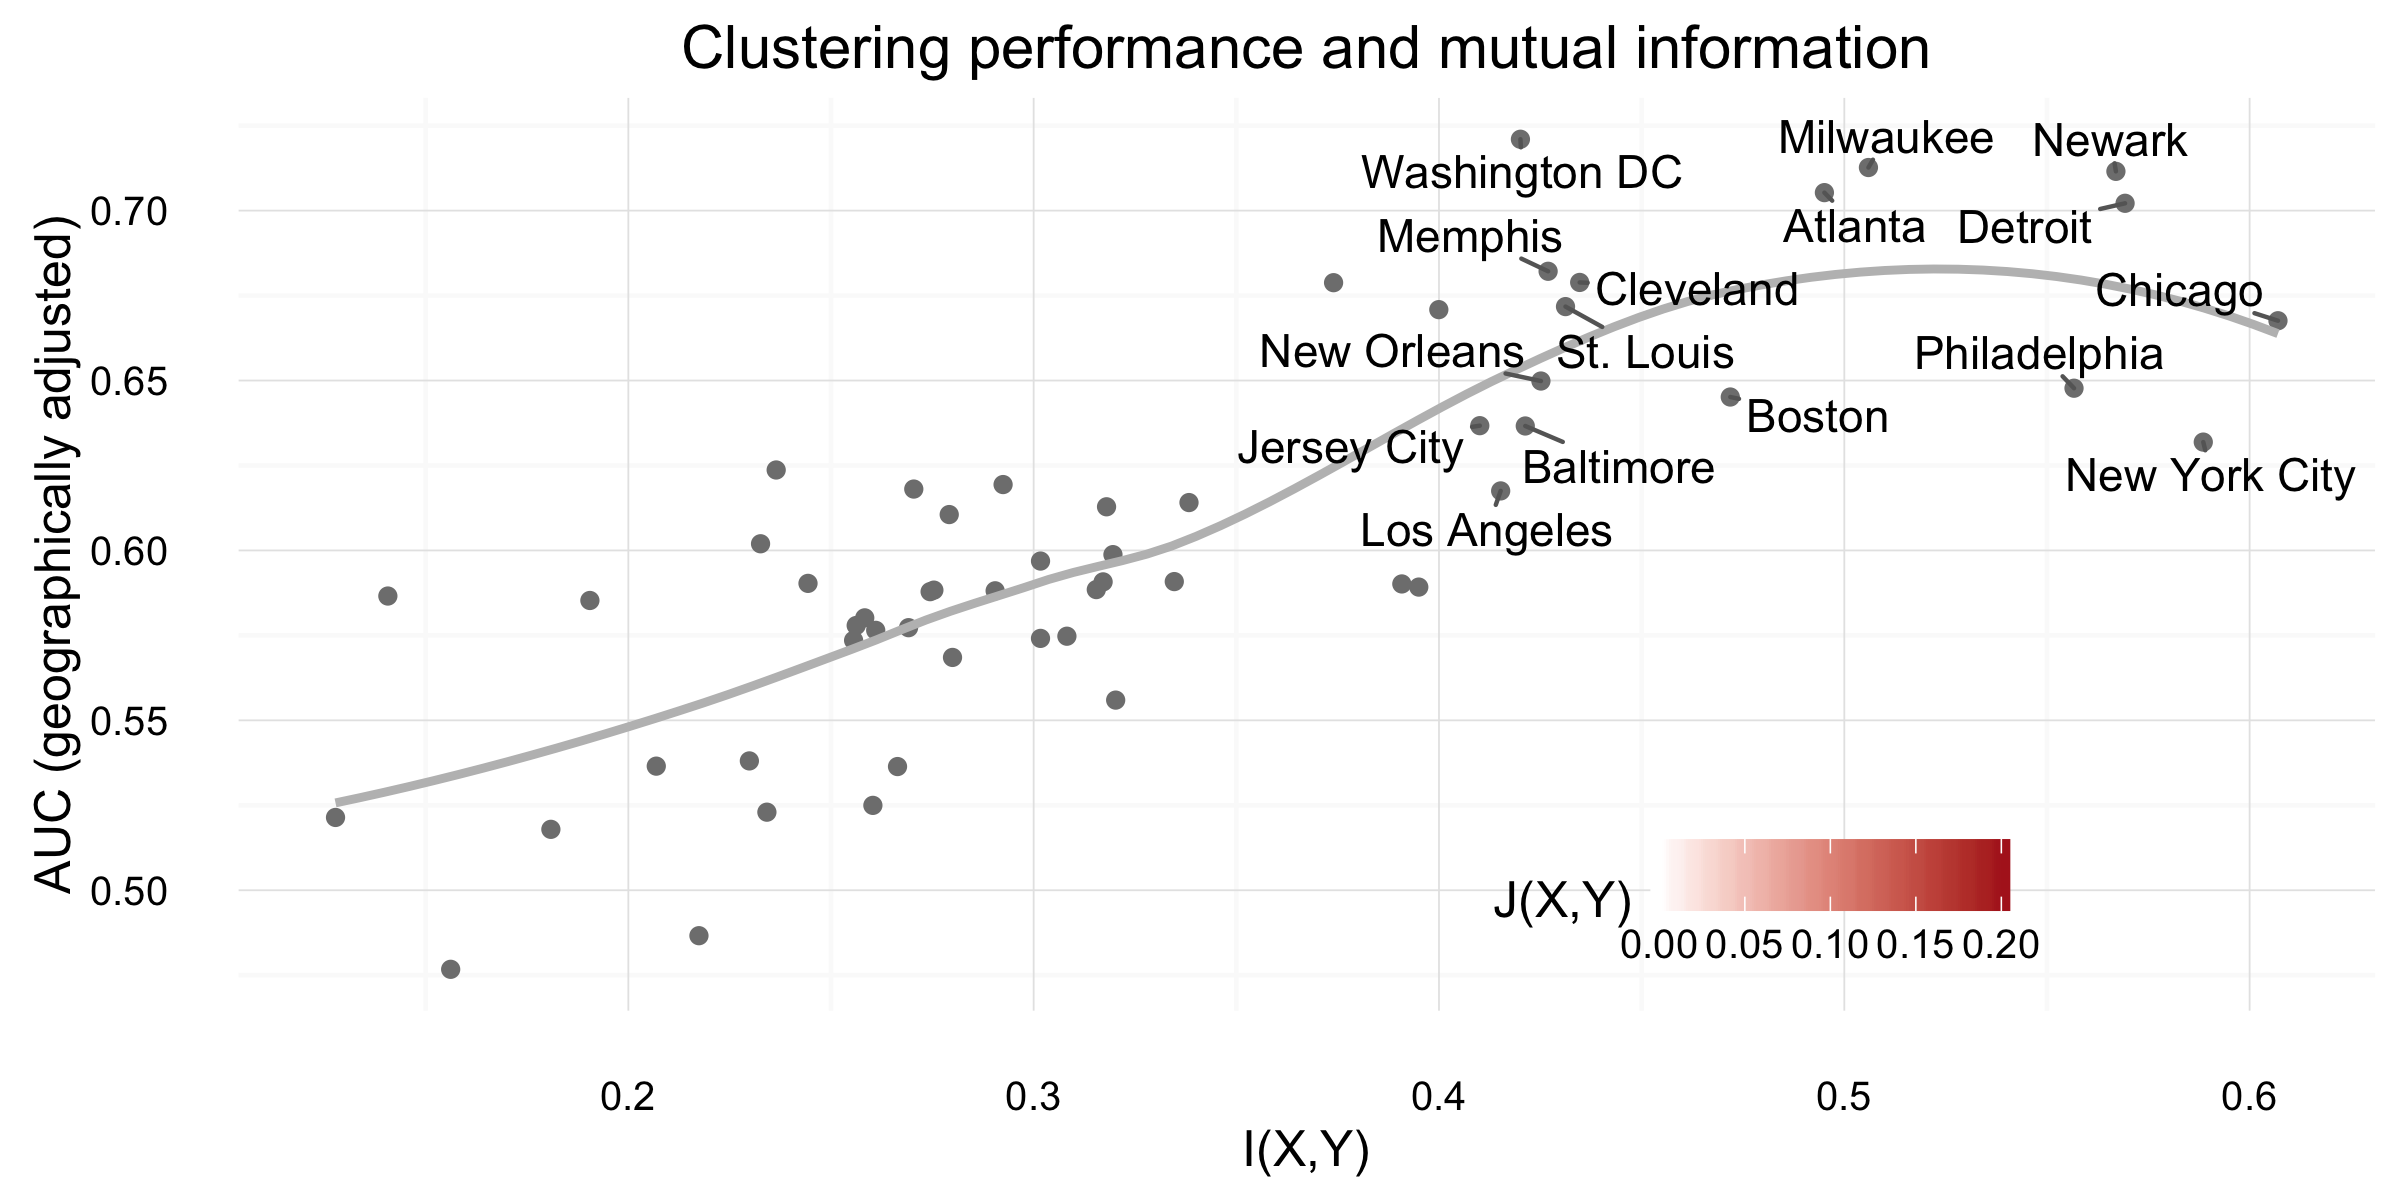
\includegraphics[width=\textwidth]{figs/info_performance_adjed.png}
		\input{figs/adjusted_regression.txt}

		\caption{Summary of regression of the clustering AUC on information measures $H(Y)$, $I(X,Y)$, $J(X,Y)$. The AUC has been geographically adjusted to account for cities like New York, whose Census blockgroups form eight disconnected components, which would mildly distort results without adjustment. Table produced using \cite{Marek2015}}.
		\label{fig:info_and_clusters}
	\end{figure}		

	Based on our discussion so far, we would expect that the AUC is related to the information measure $J(X,Y)$. Figure \ref{fig:info_and_clusters} confirms this expectation. Overall, two factors explain much about the ``clusterability'' of a city as measured by the AUC. The most important factor is the overall mutual information $I(X,Y)$. This reflects a simple intuition: when there is little spatial variation, there is not much to cluster. The second factor is the mean local information $J(X,Y)$, reflecting that spatial complexity makes clustering harder. A simple linear regression makes these insights precise. As predictors of the AUC, both $I(X,Y)$ and $J(X,Y)$ are highly significant, and the coefficient of $J(X,Y)$ is negative. The two measures jointly account for an adjusted 70\% of the variation in AUC. 
\section{Discussion}
	We have presented an information-theoretic framework for conceptualizing three core dimensions of urban diversity. Entropy measures global diversity; mutual information measures spatial evenness; and local information measures spatial exposure. Using information-based agglomerative clustering, we have also shown that these three measures are intimately related to the fineness of neighborhood structure. As \ref{fig:info_and_clusters} indicates, cities whose neighborhood structure can be easily characterized with just a few clusters tend to be those with either low diversity $H(Y)$ or low spatial exposure $J(X,Y)$, like Detroit. Cities with finer-grained spatial structure tend to have higher diversity $H(Y)$ and greater spatial exposure $J(X,Y)$, like Philadelphia. These tools are emminently practical; allowing both for the quantitative comparison of diversity profiles between cities (Figure \ref{fig:info_cross}) and more detailed analysis within a single city using naturally-defined neighborhoods (Figures \ref{fig:cluster_map} and \ref{fig:clusters}). We conclude by noting some areas for future work, and some intriguing system properties illuminated by our findings. 

While we have presented our information-theoretic framework in the context of racial residential segregation, these methods are substantially more general. Generalizing from race, information-theoretic methods applicable to any categorical variable or combinations thereof. It would be simple to conduct similar analysis for e.g. occupation type, or even to for a combination of race and occupation type. Information methods are somewhat less applicable in the case of continuous indicators \cite{Cover1991}. However, even in this case it would be possible to define interpretable qualitative categories such as \{``working class'', ``middle class'', ``upper class''\} and proceed with analysis. 

Generalizing from space, the remaining dimension of sociological interest is time. Many adults spend less than half of their waking hours at home \cite{employment_stats}, indicating that residential segregation is only a partial characterization of city-wide diversity. Fortunately, our ability to learn about daily patterns of human mobility is progressing at a rapid pace. Recent years have seen an enormous increase in the use of mobile devices, allowing the passive collection of digital traces. These traces can be processed, analyzed, and validated to derive insight into daily activity patterns \cite{Widhalm2015,Yang,Jiang2013,Jiang2012c}. In the context of these developments, the information-theoretic suite of tools is attractive in its generality. Given appropriate data, only minimal mathematical changes are necessary: 
\begin{itemize} 
	\item The entropy $H(Y)$ remains unchanged. 
	\item Spatiotemporal evenness is the degree to which spatiosocial distributions change throughout the day. It can be measured by the global spatiotemporal mutual information $I([T,X];Y)$ between time $T$, space $X$, and demographics $Y$. Also of interest is the quantity $I(X,Y|T=t)$, which measures spatial unevenness at a given time of day $t$. 
	\item The local information $J(T,X,Y)$ retains its primary definition, but now splits into two parts:  $J(T,X,Y) = J(T,Y) + J(X,Y)$. The first term on the right measures how rapidly racial trends at fixed locations change with time, while the second term is the familiar (spatial) local information. 
\end{itemize}
It is also possible to define a greedily information-maximizing spatiotemporal clustering algorithm. Such an algorithm may be of special interest in temporal analysis on longer time-scales. For example, given many years of Census data, spatiotemporal clustering would allow the identification of neighborhoods and a characterization of their demographic and spatial evolutions. 

The scaling relationship between the local information $J(X,Y)$ and the population density as shown in Figure \ref{fig:density} also deserves further investigation. Keeping in mind that $J(X,Y)$ measures the fineness of neighborhood structure, the upshot of Figure \ref{fig:density} is that, controlling for evenness, denser cities tend to have more racially-distinct neighborhoods per area. While further analysis is necessary to make this observation precise, it is intriguing to postulate a dynamical process of racial neighborhood formation and growth common to many American cities. It may be, for example, that an explanation is possible in terms of the interplay between spatial preferential attachment and infrastructure constraints. 

\bibliography{/Users/phil/bibs/library.bib}{}
\bibliographystyle{plain}
	
\section{Appendix}
	
\subsection*{Software} 

  We are pleased to make available two software repositories accompanying this analysis. 
  \begin{itemize}
    \item Package 
    \texttt{compx} for the \texttt{R} programming language implements computation of the information measures $H(Y)$, $I(X,Y)$, and $J(X,Y)$, as well as a method for information-theoretic clustering. Access \texttt{compx} at 
    \begin{displayquote}
      \texttt{https://github.com/PhilChodrow/compx}. 
    \end{displayquote}
    To install in \texttt{R}, install the package \texttt{devtools} at 
    \begin{displayquote}
    \texttt{https://cran.r-project.org/web/packages/devtools/index.html}
    \end{displayquote}
     and run the command 
    \begin{displayquote}
      \texttt{devtools::install\_github(``PhilChodrow/compx'')}
    \end{displayquote}
    in the \texttt{R} console. 
    \item The analysis repository for this project, including data acquisition and processing; core computations; and figure generation. We hope that this repository will provide useful examples of how to use \texttt{compx} for others aiming to replicate and extend our results. Download the project files at 
    \begin{displayquote}
      \texttt{https://github.com/PhilChodrow/spatial\_complexity}. 
    \end{displayquote}
  \end{itemize}

\subsection*{Relation of mutual and Fisher informations}
	Let $X$ be a continuous random variable taking values in $\R^n$, and let $Y$ be a discrete random variable define on finite alphabet $\mathcal{Y}$. Suppose further that $p(y|x) > 0$ and that $p(y|x)$ is differentiable as a function of $x$ for all $x,y \in \R^n \times \mathcal{Y}$. Fix $x_0 \in \R^n$, and define $B_r \triangleq B_r(x_0) = \{ x \in R^n \;|\; \norm{x - x_0} \leq r \}$. Additionally, define the \emph{local mutual information} in $B_r$ as the mutual information between $X$ and $Y$ where $X$ is restricted to $B_r$:
	\begin{align}
		I_r(x_0) &\triangleq \E_X[D[p(\cdot|X)\| p(\cdot|X \in B_r)]|X \in B_r] \\
		&= \int_{B_r} p(x|X \in B_r) D[p(\cdot|x)\| p(\cdot|X \in B_r)] d^n x\;.
	\end{align}
	where $D[p\|q] \triangleq \sum_{y} p(y) \log \frac{p(y)}{q(y)}$ is the Kullback-Leibler divergence of $q$ from $p$. 

	\begin{thm} \label{thm1}
		Under the stated conditions, 
		\begin{equation}
			\lim_{r\rightarrow 0} \frac{I_r(x_0)}{r^2} = \frac{n}{2(n+2)} \emph{trace}\; J_Y(x_0)\;.
		\end{equation}
		where the Fisher information matrix $J_Y$ is given by 
		\begin{align}
		J_Y(x) &\triangleq \E_Y\left[\nabla_x S_{Y}(x)\nabla_x S_{Y}(x)^T \right] \\
		S_y(x) &\triangleq \log p(y|x)\;.
	\end{align}
	\end{thm}

	The proof of Theorem \ref{thm1} proceeds by the application of a number of Taylor approximations, in tandem with a fundamental relationship of information geometry. We first expand out $I_r(x_0)$ explicitly as
	\begin{equation}
		I_r(x_0) = \int_{B_r} p(x|X \in B_r) D[p(\cdot|x)\| p(\cdot|X \in B_r)] d^n x\;. \label{eq:explicit}
	\end{equation}

	\begin{lm} \label{approximations}
		The following approximation relationships hold for the components of \eqref{eq:explicit}:
		\begin{enumerate}[label=\emph{(\alph*)}]
			\item $p(X\in B_r,Y) = p(x_0, Y) v(B_r) + O(r^{n+2})$
			\item $p(Y|X \in B_r) = p(Y|x_0) + e_y$ where the error terms $e_y$ satisfy $e_y \in O(r^{2})$ and $\sum_{y \in \mathcal{Y}} e_y = 0$. 
			\item $p(x|X \in B_r) = \frac{1 + O(r)}{v(B_r)}$
		\end{enumerate}
	\end{lm}
	\begin{proof}
		For each approximation,  we directly apply Taylor expansions about $X = x_0$. 
		\begin{enumerate}[label=(\alph*)]
			\item We have 
				\begin{align}
					p(X\in B_r, Y) &= \int_{B_r} p(x,Y) \; d^nx \\
					&= \int_{B_r} p(x_0,Y) + \frac{\partial p(x_0, Y)}{\partial x}(x - x_0) + O(\norm{x - x_0}^2) \; d^nx \\
					&= p(x_0, Y)v(B_r) +  \frac{\partial p(x_0, Y)}{\partial x} \int_{B_r} (x - x_0)\; d^nx  \\
					&\quad \quad+ O\left(\int_{B_r} \norm{x - x_0}^2\; d^nx\right) \\
					&= p(x_0, Y)v(B_r) + O(r^{n+2})\;,
				\end{align}
				where the middle term vanishes due to spherical symmetry. 
			\item The fact that the error terms $e_y$ must satisfy $\sum_{y \in \mathcal{Y}} e_y = 0$ follows from the fact that $p(Y|X \in B_r)$ must be a valid probability distribution over $\mathcal{Y}$. We'll now show that $e_y \in O(r^{ß2})$. First, 
				\begin{align}
					p(X \in B_r) &= \sum_{y\in \mathcal{Y}} p(X \in B_r, y)  \\
					&= \sum_{y\in \mathcal{Y}} \left[p(x_0, y)v(B_r) + O(r^{n+2}) \right] \\
					&= p(x_0)v(B_r) + O(r^{2});\,
				\end{align}
			from part (a). Next, 
				\begin{align}
					p(Y|X \in B_r) &= \frac{p(X\in B_r, Y)}{p(X \in B_r)} \\
					&= \frac{p(x_0, Y)v(B_r) + O(r^{n+2})}{p(x_0)v(B_r) + O(r^{n+2})} \\
					&= p(Y|x_0) + O(r^2)\;,
				\end{align}
			which completes this part of the argument. 
			\item First, 
				\begin{align}
					p(X \in B_r) &= \int_{B_r} p(x) \; d^nx  \\
					&= \int_{B_r} \left[p(x_0) + \nabla p(x_0)(x - x_0) + O(r^2)\right] \; d^nx \\ 
					&= p(x_0) v(B_r) + O(r^{n+2})\;,
				\end{align}
				where the middle term again vanishes through spherical symmetry. Thus, for $x \in B_r$, we have
				\begin{align}
					p(x | X \in B_r) &= \frac{p(x)}{p(X \in B_r)} \\
					&= \frac{p(x_0) + \nabla p(x_0)(x - x_0) + O(r^2)}{p(x_0) v(B_r) + O(r^{n+2})} \\
					&= \frac{1 + O(r)}{v(B_r)}\;.
				\end{align}
		\end{enumerate}
	\end{proof}

	\begin{lm} The following approximation holds for the divergence factor in the integral \eqref{eq:explicit}
		\begin{equation}
			D[p(\cdot|x)\| p(\cdot|X \in B_r)] = D[p(\cdot|x)\| p(\cdot|x_0)] + O(r^{3})
		\end{equation}
	\end{lm}
	\begin{proof}
		We compute directly: 
		\begin{align}
			D[p(\cdot|x)\| p(\cdot|X \in B_r)] &= \sum_{y \in \mathcal{Y}} p(y|x) \log \frac{p(y|x)}{p(y|X \in B_r)} \\
			&= - H[Y|X = x] - \sum_{y \in \mathcal{Y}} p(y|x) \log p(y|X \in B_r) \\
			&= - H[Y|X = x] - \sum_{y \in \mathcal{Y}} p(y|x) \log \left(p(y|x_0) + e_y)\right) \tag{from Lemma \ref{approximations}}\\
			&= - H[Y|X = x] - \sum_{y \in \mathcal{Y}} p(y|x) \left[\log p(y|x_0) + \frac{e_y}{p(y|x_0)} + O(e_y^2)\right] \\
			&= D[p(\cdot|x)\| p(\cdot|x_0)] + \sum_{y \in \mathcal{Y}} \frac{p(y|x)}{p(y|x_0)}  e_y \tag{quadratic terms negligible} \\
			&=D[p(\cdot|x)\| p(\cdot|x_0)] \\
			&\quad + \sum_{y \in \mathcal{Y}} \left(1 + \frac{1}{p(y|x_0)} \nabla p(y|x_0)(x - x_0) + O(r^{2})\right)    e_y \\
			&= D[p(\cdot|x)\| p(\cdot|x_0)] + \sum_{y \in \mathcal{Y}} \left[e_y + O(r^{3})\right] \tag{$e_y \in O(r^2)$}\\
			&= D[p(\cdot|x)\| p(\cdot|x_0)] + O(r^3) \tag{$\sum_{y \in \mathcal{Y}} e_y = 0$}
		\end{align}
	\end{proof}

	\begin{lm} For any positive-semidefinite matrix $A \in \R^{n\times n}$, 
		$$\int_{B_r} \left< x - x_0, A(x-x_0) \right> d^n x = \frac{n}{n+2} r^{2} v(B_r) \text{\emph{trace}} (A)$$
	\end{lm}
		
	\begin{proof}
		Since $A$ is positive-semidefinite, there exist an orthonormal matrix $P$ and a diagonal matrix $D$ such that $A = P^TDP$. Furthermore, the entries of $D$ are the eigenvalues $\{\lambda_i\}$ of $A$. Then, 
		\begin{align}
			\int_{B_r} \left< x - x_0, A(x-x_0) \right> d^n x &= \int_{B_r} \left< x - x_0, P^T DP(x-x_0) \right> d^n x\\
			&= \int_{B_r} \left< P(x - x_0),  DP(x-x_0) \right> d^n x \;.
		\end{align}
		We can regard $P$ as a reparameterization of $B_r$; since $\det P = 1$, we have 
		\begin{align}
			\int_{B_r} \left< P(x - x_0),  DP(x-x_0) \right> d^n x &= \int_{B_r} \left< x - x_0,  D(x-x_0) \right> d^n x \\
			&= r^n\int_{B_n} \left< rx, rDx \right> d^n x \\
			&= r^{n+2}\int_{B_n} \left< x, Dx \right> d^n x \;,
		\end{align}
		where $B_n$ is the unit $n$-ball. We also let $S_n(r)$ be the $n$-sphere of radius $r$. Continuing, 
		\begin{align}
			r^{n+2}\int_{B_n} \left< x, Dx \right> d^n x &= r^{n+2} \int_{B_n} \sum_{i= 1}^n x_i^2 \lambda_i \; d^nx \\
			&= r^{n+2} \sum_{i = 1}^n \lambda _i \int_{B_n} x_i^2 \; d^nx \\
			&= \frac{r^{n+2}}{n} \sum_{i = 1}^n \lambda _i \int_{B_n} \norm{x}^2 \; d^nx \\ \tag{spherical symmetry} \\
			&= \frac{r^{n+2}}{n} \text{trace}(A)  \int_{B_n} \norm{x}^2 \; d^nx \\ \tag{spherical symmetry} \\
			&= \frac{r^{n+2}}{n} \text{trace} (A) \int_{\rho \in [0,1]} \rho^2 S_{n-1}(\rho) d\rho \\
			&= \frac{r^{n+2}}{n} \text{trace} (A) \int_{\rho \in [0,1]} \rho^{n+1} S_{n-1}(1) d\rho \\
			&= \frac{r^{n+2}}{n} \text{trace} (A)  \frac{1}{n+2} S_{n-1}(1) \\
			&= \frac{r^2}{n+2}  \text{trace} (A)  n r^{n}v(B_n(1)) \\
			&= \frac{n}{n+2} r^{2} v(B_r) \text{trace} (A)\;,
		\end{align}
		as was to be shown. 
	\end{proof}

	\begin{fct*}
		The Kullback-Leibler divergence and the Fisher information $J_Y$ are related according to the approximation 
		\begin{equation}
			D[p(\cdot|x)\| p(\cdot|x_0)] = \frac{1}{2}\left<x - x_0, J_Y(x_0)(x - x_0) \right> + O(\norm{x - x_0}^3)
		\end{equation}
	\end{fct*}

	We are finally ready to prove Theorem \ref{thm1}. Computing directly, we have 
	\begin{align}
		I_r(x_0) &\triangleq \E_X[D[p(\cdot|X)\| p(\cdot|X \in B_r)]|X \in B_r]\;. \\
		&= \int_{B_r} p(x|X \in B_r) D[p(\cdot|x)\| p(\cdot|X \in B_r)] d^n x \\
		&= \int_{B_r} \left[\frac{1 + O(r)}{v(B_r)}\right] D[p(\cdot|x)\| p(\cdot|X \in B_r)] d^n x \tag{Lemma 1(c)}\\ 
		&= \left[\frac{1 + O(r)}{v(B_r)}\right]\int_{B_r}  \left(D[p(\cdot|x)\| p(\cdot|x_0)] + O(r^{3})\right) d^n x \tag{Lemma 2}\\
		&= \left[\frac{1 + O(r)}{v(B_r)}\right]\int_{B_r} \left( \frac{1}{2}\left<x - x_0, J_Y(x_0)(x - x_0) \right> + O(\norm{x - x_0}^3) + O(r^{3})\right) d^n x \\
		&= \frac{1}{2}\left[\frac{1 + O(r)}{v(B_r)}\right]\int_{B_r} \left(\left<x - x_0, J_Y(x_0)(x - x_0) \right> + O(r^{3})\right) d^n x \\
		&= \frac{1}{2}\left[\frac{1 + O(r)}{v(B_r)}\right]\left(\frac{n}{n+2} r^{2} v(B_r) \text{trace} (J_Y(x_0)) + v(B_r)O(r^{3})\right) \\
		&= r^2\frac{n}{2(n+2)}\left[1 + O(r)\right]\left(\text{trace} (J_Y(x_0)) + O(r^{3})\right)\;.
	\end{align}
	Dividing through by $r^2$ and computing the limit as $r \rightarrow 0$ proves the result. 


\subsection*{Computational Methods and Assumptions}
	In this section, we provide a specification of the computational procedure used to estimate $J(X,Y) = \E_x[J_Y(X)]$ using blockgroup level data from the U.S. Census. 

	For fixed Census blockgroup $i$, let $P_i$ be the population, let $A_i$ be the area, let $\rho_i = P_i / A_i$ be the population density, and let $p^i_Y(y)$ be the observed proportion of racial group $y$. For hex $k$ in our hexagonal grid, let $N_k$ be the set of overlapping Census blockgroups. We also define $p^{k}_I(i) = \rho_i / \sum_{i \in N_k} \rho_i$ as the estimated proportion of population within hex $k$ residing in blockgroup $i$. This definition embodies a computationally-simplifying assumption that each blockgroup in $N_k$ overlaps hex $k$ with equal area. Finally, $p^k_Y(y) = \sum_{i \in N_k} p^{k}_I(i) p^i_Y(y)$ is the estimated overall racial composition of hex $k$. Then, we estimate the mutual information in hex $k$ as 
	\begin{equation}
		I(k) = \sum_{i \in N_k} p^k_I(i) D[p^i_Y(\cdot) \| p^k_Y(\cdot)]\;. 
	\end{equation}
	Using \eqref{eq:approx}, the estimated Fisher information is 
	\begin{equation}
		J(k) \approx \frac{4 I(k)}{r^2}
	\end{equation}
	where $r$ is the grid radius. The estimated population in hex $k$ is $P_k = A_k\sum_{i \in N_k} \rho_i$, where $A_k$ is the cell area. We finally estimate $\E_X[J(X)]$ as 
	\begin{equation}
		J(X,Y) = \E_X[J_Y(X)] \approx \frac{1}{\sum_k P_k} \sum_k P_k J(k)
	\end{equation}


\subsection{Specification of Spatially-Constrained Information-Theoretic Clustering}
	

\end{document}


% Todo: 
% Reframe the language: "neighborhoods" is probably not right.
% Focus the argument. Our core claims are: 
% 	1. We have at least three concepts here, so please use at least three measures. 
%   2. A good set of measures to use are grounded in information theory, since they talk nicely to each other, have good properties, and are operationally interpretable. 
%   3. 









